\documentclass[10pt]{beamer}
\usetheme{metropolis}
% all imports
\usepackage[utf8]{inputenc}
\usepackage[T1]{fontenc}
\usepackage{lmodern}
\usepackage{appendixnumberbeamer}
\usepackage{hyperref}
\usepackage{booktabs}
\usepackage{bm}
\usepackage[scale=2]{ccicons}
\usepackage[outputdir=build]{minted}
\usepackage{pgfplots}
\usepackage{array,colortbl,xcolor}
\usepgfplotslibrary{dateplot}
\usepackage{setspace}
\usepackage{etoolbox}
\usepackage{xspace}
\usepackage{tikz}
\usetikzlibrary{shapes,arrows,positioning,fit,backgrounds}
\usepackage{tkz-euclide}
\usepackage{multirow}

\AtBeginEnvironment{quote}{\singlespacing}

\AtBeginEnvironment{quote}{\singlespacing}

% new commands
\newcommand{\themename}{\textbf{\textsc{metropolis}}\xspace}
\newcommand{\vect}[1]{\bm{#1}}
\newcommand{\myprime}[1]{{#1}^{\prime}}
\newcommand{\grad}[2]{\nabla_{#1} {#2}}
\newcommand{\dotp}[2]{{#1}^{\top}{#2}}
\newcommand{\dotpPright}[2]{{#1}^{\top}\left({#2}\right)}
\newcommand{\outerp}[2]{\left({#1}\right){#2}^{\top}}
\newcommand{\Jacobian}[2]{\frac{\partial #1}{\partial #2}}
\newcommand{\Vocab}{\mathbb{V}}
\DeclareMathOperator*{\argmin}{arg\,min}

% definitions
\definecolor{blue}{RGB}{159, 192, 176}
\definecolor{green}{RGB}{160, 227, 127}
\definecolor{orange}{RGB}{243, 188, 125}
\definecolor{red}{RGB}{253, 123, 84}
\definecolor{nephritis}{RGB}{39, 174, 96}
\definecolor{emerald}{RGB}{46, 204, 113}
\definecolor{turquoise}{RGB}{39, 174, 96}
\definecolor{green-sea}{RGB}{22, 160, 133}
\definecolor{purple}{RGB}{181, 124, 215}
% Tikzstyles for Computation Graphs

% nodes
\tikzstyle{noop} = [circle, draw=none, fill=red, minimum size = 10pt]
\tikzstyle{op} = [circle, draw=red, line width=1.5pt, fill=red!70, text=black, text centered, font=\bf \normalsize, minimum size = 25pt]

\tikzstyle{opintense} = [circle, draw=red, line width=1.5pt, fill=red!150, text=black, text centered, font=\bf \normalsize, minimum size = 25pt]


%new style
\tikzstyle{gp} = [circle, draw=red, line width=4pt, text=black, text centered, font=\bf \normalsize, minimum size = 4.cm]

\tikzstyle{box} = [rectangle, draw=red, line width=1.5pt, fill=red!70, text=black, align=center, font=\bf \normalsize, minimum size = 45pt]

\tikzstyle{state} = [circle, draw=blue, line width=1.5pt, fill=blue!70, text=black, text centered, font=\bf \normalsize, minimum size = 25pt]

\tikzstyle{output} = [circle, draw=purple, line width=1.5pt, fill=purple!70, text=black, text centered, font=\bf \normalsize, minimum size = 25pt]


\tikzstyle{gradient} = [circle, draw=nephritis, line width=1.5pt, fill=nephritis!60, text=black, text centered, font=\bf \normalsize, minimum size = 25pt]
\tikzstyle{textonly} = [draw=none, fill=none, text centered, font=\bf \normalsize]
\tikzstyle{boxtextonly} = [draw=none, fill=none, align=center, font=\bf \normalsize]

\tikzstyle{normal} = [circle, draw=black, line width=1.0pt, fill=none, text=black, text centered, font=\bf \normalsize, minimum size = 20pt]


% edges
\tikzstyle{tedge}  = [draw, thick, >=latex, ->]
\tikzstyle{tedge_dashed}  = [draw, thick, >=latex, ->, dashed]
\tikzstyle{nedge}  = [draw, thick, >=latex]
\tikzstyle{nedge_dashed}  = [draw, thick, >=latex, dashed]


% namedscope
\tikzstyle{namedscope} = [circle, draw=orange, line width=1.5pt, fill=orange!60, align=center, inner sep=0pt]

\title{Aprendizado de Máquina em Linguagem Natural}
\date{\today}

\author{
  Beatriz Albiero\\
  \url{https://www.linkedin.com/in/beatriz-albiero-765953a5/}
  \vspace{0.1 cm}
  \and\\ 
  Felipe Salvatore\\
  \url{https://felipessalvatore.github.io/}
  \vspace{0.1 cm}
  \and\\
}

\institute{\textbf{USP}:University of São Paulo}


\begin{document}
\nocite{DeepLearningbook}
\maketitle

\section{Conceitos básicos}

\begin{frame}{Introdução a aprendizado de máquina}
\begin{figure}[ht!]
\centering
\scalebox{1.3}{
\begin{tikzpicture}[auto]

\node[boxtextonly] (message) {Um algoritimo de \alert{aprendizado de máquina}\\ é um algoritmo que é capaz \\de usar dados para \\realizar uma tarefa};

\node[textonly, below = 30pt of message] (inv) {};


\node[textonly, left= 20pt of inv] (reg) {Regressão};

\node[textonly, below= 3pt of reg] (x1) {$\vect{x}_1, \dots, \vect{x}_N$};

\node[textonly, below= 40pt of x1] (y1) {$y_1, \dots, y_N$};


\node[textonly, right= 30pt of inv] (class) {Classificação};

\node[textonly, below= 3pt of class] (x2) {$\vect{x}_1, \dots, \vect{x}_N$};

\node[textonly, below= 40pt of x2] (y2) {$L_1, \dots, L_N$};


%edges
\draw[tedge, orange!120, line width=1mm]  (x1) -- (y1);
\draw[tedge, orange!120, line width=1mm]  (x2) -- (y2);



\end{tikzpicture}
} % scalebox
\end{figure}


\end{frame}

\begin{frame}{Regressão}
\begin{center}
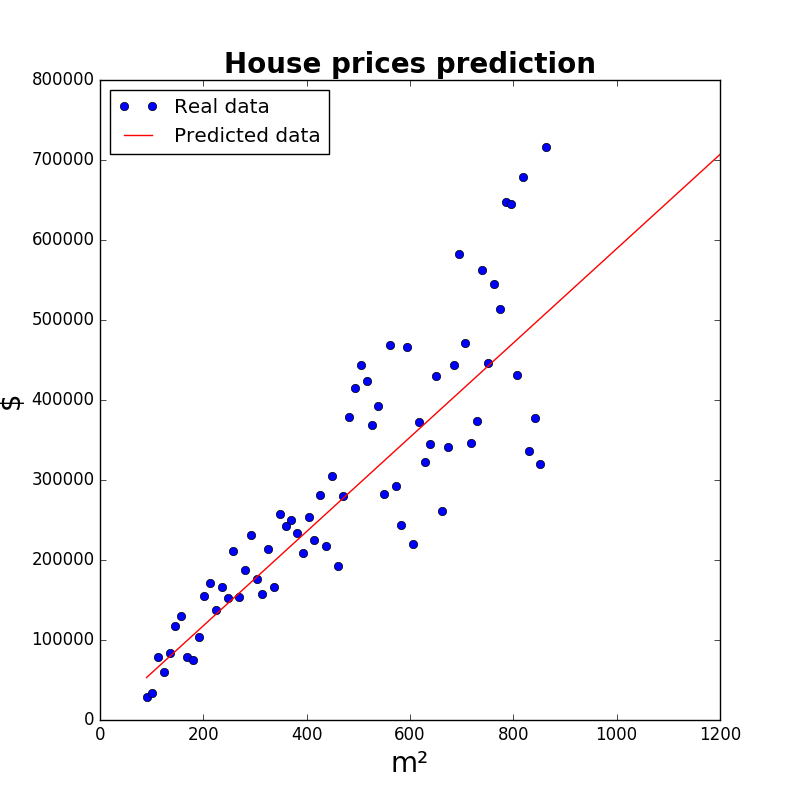
\includegraphics[scale=0.40]{images/house_prices.png}
\end{center}
\end{frame}


\begin{frame}{Classificação: Fashion MNIST \cite{xiao2017/online}}
\begin{figure}[ht!]
\centering

\scalebox{1.05}{
\begin{tikzpicture}[auto]

% operations =============================

% nodes
\node (shirt)
    {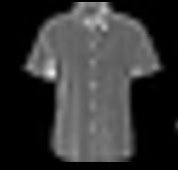
\includegraphics[width=.15\textwidth]{images/shirt.png}};
\node[textonly, below=1pt of shirt] (dimension0) {{\small$28\times 28$}};
\node[textonly, above right= 10pt and 90pt of shirt] (vector) {$\begin{bmatrix}0.34\\ \vdots \\0.06\end{bmatrix}$};
\node[textonly, above=1pt of vector] (x) {$\vect{x}$};
\node[textonly, below=1pt of vector] (dimension1) {{\small$784\times 1$}};

\node[textonly, below=30pt of vector] (y) {$y=1$};

\node[textonly, below=30pt of y] (one-hot) {$\begin{bmatrix}1\\ \vdots \\0\end{bmatrix}$};

\node[textonly, above=1pt of one-hot] (yvector) {$\vect{y}$};
\node[textonly, below=1pt of one-hot] (dimension2) {{\small$10\times 1$}};



% edges
\path[tedge, orange!120, line width=1mm]  (shirt) -- (vector);
\path[tedge, orange!120, line width=1mm] (shirt) -- (y);
\path[tedge, orange!120, line width=1mm] (shirt) -- (one-hot);



\end{tikzpicture}
} % scalebox
\end{figure}

\end{frame}


\begin{frame}{Aprendizado por redes neurais}

O que sabemos sobre o cérebro:
\vspace{0.2cm}
\begin{itemize}
\item neurônios em rede
\vspace{0.2cm}
\item  neurônios emitem sinais elétricos (disparam)
\vspace{0.2cm}
\item dendritos e axônios


\end{itemize}

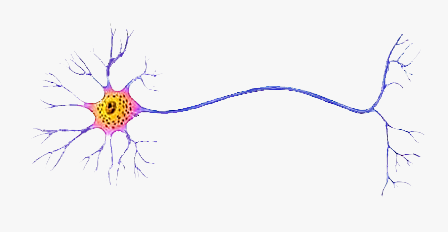
\includegraphics[width=.50\textwidth]{images/neuron.png}
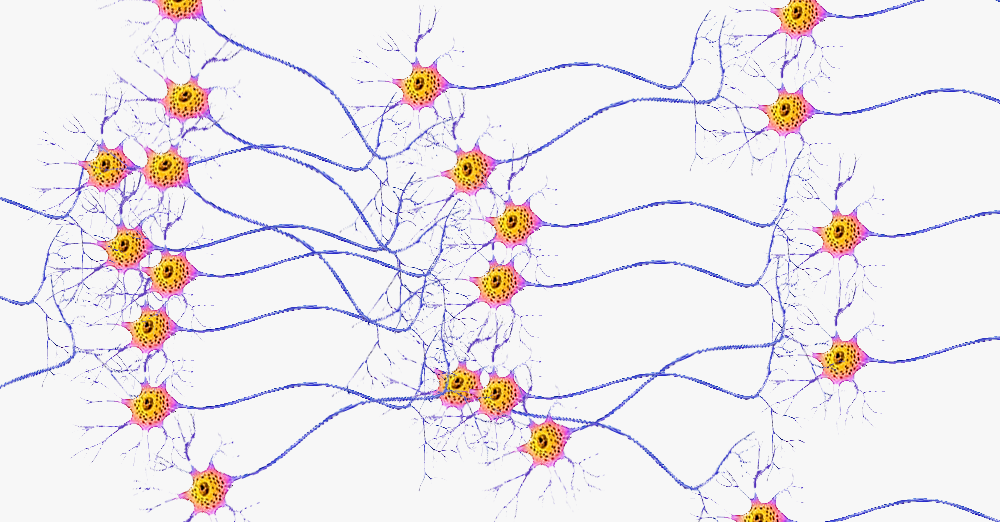
\includegraphics[width=.50\textwidth]{images/neuronsnetwork.png}
\\
\\
\footnotesize{imagem retirada de \cite{metodosupera}}


\end{frame}



\begin{frame}{Aprendizado por Redes Neurais}

Traduzindo para o modelo de redes neurais artificiais:
\vspace{0.2cm}
\begin{itemize}
\item Energia recebida: \alert{Inputs}
\vspace{0.2cm}
\item  Energia enviada: \alert{Output}
\vspace{0.2cm}
\item  Força entre uma conexão e outra: \alert{Peso ($\vect{\theta}$)}
\vspace{0.2cm}

\item Carga mínima: \alert{Threshold}
\vspace{0.2cm}
\item Uma função que recebe um input e emite um output mas leva em consideração um threshold mínimo: \alert{Função de ativação}

\end{itemize}

\end{frame}



\begin{frame}{Função de ativação: função sigmoid}
\begin{figure}[ht!]
\centering

\scalebox{1.0}{
\begin{tikzpicture}
    \begin{axis}%
    [
        grid=major,     
        xmin=-6,
        xmax=6,
        axis x line=bottom,
        ytick={0,.5,1},
        ymax=1,
        axis y line=middle,
    ]
        \addplot%
        [	orange!180,
        	ultra thick,
%             blue,%
            mark=none,
            samples=100,
            domain=-6:6,
        ]
        (x,{1/(1+exp(-x))});
    \end{axis}
\node[textonly] (sigmoid) at (8.75,2.8) {{\Large$\sigma(x) = \frac{1}{1 + e^{-x}}$}};
\end{tikzpicture}
} % scalebox
\end{figure}
\end{frame}

\begin{frame}{função de ativação: ReLU (Rectified Linear Unit)}
\begin{figure}[ht!]
\centering

\scalebox{1.0}{
\begin{tikzpicture}
    \begin{axis}%
    [
        grid=major,     
        xmin=-6,
        xmax=6,
        axis x line=bottom,
        ytick={0},
        ymax=10,
        axis y line=middle,
    ]
        \addplot%
        [	orange!180,
        	ultra thick,
%             blue,%
            mark=none,
            samples=100,
            domain=-6:6,
        ]
        (x,{max(x,0)});
    \end{axis}
\node[textonly] (relu) at (8.95,2.8) {{\Large$g(x) = max\{0,x\}$}};
\end{tikzpicture}
} % scalebox
\end{figure}
\end{frame}

\begin{frame}[fragile]{Perceptron}
\begin{figure}[ht!]
\centering

\scalebox{1.15}{
\begin{tikzpicture}[auto]
%operations=========================

\node[textonly] (x1) {input 1};
\node[textonly, below=0.01pt of x1] (x11) {$x_1$};
\node[textonly, below=45pt of x1] (x2) {input 2};
\node[textonly, below=0.01pt of x2] (x22) {$x_2$};
\node[textonly, below=45pt of x2] (x3) {input 3};
\node[textonly, below=0.01pt of x3] (x33) {$x_3$};

\node[gp, right=25pt of x2] (vk) {};
\node[textonly, right=40pt of vk] (yk) {$output$};
\node[textonly, above=-9pt of vk] (inv1) {};
\node[textonly, below=-9pt of vk] (inv2) {};
\node[boxtextonly, right=40pt of x2] (soma) {soma\\dos\\inputs};
\node[boxtextonly, right=12pt of soma] (sigmoid) {sigmóide\\da\\soma};



% edges
\path[tedge] (x1) edge node[above=1.8pt] {$\theta_{1}$} (vk);
\path[tedge] (x2) edge node[above=0.2pt] {$\theta_{2}$} (vk);
\path[tedge] (x3) edge node[above=3pt] {$\theta_{3}$} (vk);
\path[tedge] (vk) edge node[above=1pt] {}  (yk) ;]
\path[nedge, draw=red, line width=4pt] (inv1) --  (inv2) ;

\end{tikzpicture}
} % scalebox
\end{figure}
\end{frame}

\begin{frame}[fragile]{Perceptron}
\begin{figure}[ht!]
\centering

\scalebox{1.15}{
\begin{tikzpicture}[auto]

% operations =============================
\node[op] (x2) {$x_2$};
\node[op, above=40pt of x2] (x1) {$x_1$};
\node[op, below=40pt of x2] (x3) {$x_3$};
\node[op, right=60pt of x2] (vk) {$v$};
\node[op, right=40pt of vk] (yk) {$\hat{y}$};
\node[textonly, below right=20pt of x3] (Synaptic) {Synaptic link};
\node[textonly, below right=50pt of vk] (Activation) {Activation link};
\node[textonly, above right=28pt and -46pt of yk] (f) {$\hat{y} = f(\vect{x};\vect{\theta})= g\left(\sum_{i=1}^{3} \theta_ix_i\right)$};


% edges
\path[tedge] (x1) edge node[above=1.8pt] {$\theta_{1}$} (vk);
\path[tedge] (x2) edge node[above=0.2pt] {$\theta_{2}$} (vk);
\path[tedge] (x3) edge node[above=3.8pt] {$\theta_{3}$} (vk);
\path[tedge] (vk) edge node[above=1pt] {{\Large$g$}}  (yk) ;

% info edges
\draw[orange!120, line width=1mm]  (Synaptic) to [out=150,in=0] (x3);
\draw[orange!120, line width=1mm] (Synaptic) to [out=150,in=-100] (vk);

\draw[orange!120, line width=1mm]  (Activation) to [out=170,in=-40] (vk);
\draw[orange!120, line width=1mm] (Activation) to [out=170,in=-100] (yk);



\end{tikzpicture}
} % scalebox
\end{figure}

\end{frame}

\begin{frame}[fragile]{Multi layer perceptron -- Feedforward neural network}
\begin{figure}[ht!]
\centering

\scalebox{1.12}{
\begin{tikzpicture}[auto]

% operations =============================
\node[op] (x2) {$x_2$};
\node[op, above=60pt of x2] (x1) {$x_1$};
\node[op, below=60pt of x2] (x3) {$x_3$};
\node[op, right=80pt of x2] (v1) {$v_1$};
\node[op, below=20pt of v1] (v2) {$v_2$};

\node[op, right=40pt of v1] (y1) {$\hat{y}_{1}$};
\node[op, right=40pt of v2] (y2) {$\hat{y}_{2}$};

\node[textonly, above right=28pt and -86pt of y1] (f) {$\vect{\hat{y}} = f(\vect{x};\vect{\theta})= g(\vect{v})= g(\vect{\theta} \vect{x})$};


% edges
\path[tedge] (x1) edge node[above=1.8pt] {$\vect{\theta}_{1,1}$} (v1);
\path[tedge] (x2) edge node[above=0.2pt] {$\vect{\theta}_{1,2}$} (v1);
\path[tedge] (x3) edge node[above=3.8pt] {$\vect{\theta}_{1,3}$} (v1);
\path[tedge] (v1) edge node[above=1pt] {{\Large$g$}}  (y1) ;
\path[tedge] (x1) edge node[above=1.8pt] {$\vect{\theta}_{2,1}$} (v2);
\path[tedge] (x2) edge node[above=0.2pt] {$\vect{\theta}_{2,2}$} (v2);
\path[tedge] (x3) edge node[above=3.8pt] {$\vect{\theta}_{2,3}$} (v2);
\path[tedge] (v2) edge node[above=1pt] {{\Large$g$}}  (y2) ;

% info edges



\end{tikzpicture}
} % scalebox
\end{figure}

\end{frame}

\begin{frame}[fragile]{Multi layer perceptron -- Feedforward neural network}
\begin{figure}[ht!]
\centering

\scalebox{0.9}{
\begin{tikzpicture}[auto]

% operations =============================
\node[op] (x2) {$x_2$};
\node[op, above=60pt of x2] (x1) {$x_1$};
\node[op, below=60pt of x2] (x3) {$x_3$};
\node[op, right=80pt of x2] (v1) {$v_1$};
\node[op, below=20pt of v1] (v2) {$v_2$};

\node[op, right=40pt of v1] (h1) {$h_{1}$};
\node[op, right=40pt of v2] (h2) {$h_{2}$};

\node[op, right=40pt of h1] (z1) {$z_{1}$};
\node[op, right=40pt of h2] (z2) {$z_{2}$};


\node[op, right=40pt of z1] (y1) {$\hat{y}_{1}$};
\node[op, right=40pt of z2] (y2) {$\hat{y}_{2}$};

\node[textonly, above right=38pt and -86pt of h1] (f) {$\vect{\hat{y}} = f(\vect{x};\vect{\theta})= g_2(\vect{V}\vect{h})= g_2(\vect{V}g_1(\vect{W}\vect{x}))$};


% edges input to hidden1
\path[tedge] (x1) edge node[above=1.8pt] {$\vect{W}_{1,1}$} (v1);
\path[tedge] (x2) edge node[above=0.2pt] {$\vect{W}_{1,2}$} (v1);
\path[tedge] (x3) edge node[above=3.8pt] {$\vect{W}_{1,3}$} (v1);

\path[tedge] (x1) edge node[above=1.8pt] {$\vect{W}_{2,1}$} (v2);
\path[tedge] (x2) edge node[above=0.2pt] {$\vect{W}_{2,2}$} (v2);
\path[tedge] (x3) edge node[above=3.8pt] {$\vect{W}_{2,3}$} (v2);

% edges activation1
\path[tedge] (v1) edge node[above=1pt] {{\Large$g_1$}}  (h1) ;
\path[tedge] (v2) edge node[above=1pt] {{\Large$g_1$}}  (h2) ;

% edges input to hidden2
\path[tedge] (h1) edge node[above=1.8pt] {$\vect{V}_{1,1}$} (z1);
\path[tedge] (h2) edge node[below left=-4.2pt and 4.5pt] {$\vect{V}_{2,1}$} (z1);

\path[tedge] (h1) edge node[above=1.8pt] {$\vect{V}_{1,2}$} (z2);
\path[tedge] (h2) edge node[above=0.2pt] {$\vect{V}_{2,2}$} (z2);

% edges activation2
\path[tedge] (z1) edge node[above=1pt] {{\Large$g_2$}}  (y1) ;
\path[tedge] (z2) edge node[above=1pt] {{\Large$g_2$}}  (y2) ;


% info edges



\end{tikzpicture}
} % scalebox
\end{figure}

\end{frame}

\begin{frame}[fragile]{Multi layer perceptron -- Feedforward neural network}
\begin{figure}[ht!]
\centering

\scalebox{1.3}{
\begin{tikzpicture}[auto]

% operations =============================

% input layer
\node[op] (x3) {$x_3$};
\node[op, above=20.5pt of x3] (x2) {$x_2$};
\node[op, above=20.5pt of x2] (x1) {$x_1$};

% hidden layer
\node[op,  below right= 10pt and 90pt of x2] (h2) {$h_2$};
\node[op, above=20.5pt of h2] (h1) {$h_1$};

% output layer
\node[op,  right=50pt of h1] (out1) {$\hat{y}_1$};
\node[op,  right=50pt of h2] (out2) {$\hat{y}_2$};

%labels

\node[textonly,  above right= 30pt and 30pt of x2] (W) {\LARGE{$\vect{W}$}};

\node[textonly,  above right= 40pt and 15pt of h2] (U) {\LARGE{$\vect{U}$}};



%edges input to hidden

\path[tedge] (x1) -- (h1);
\path[tedge] (x1) -- (h2);


\path[tedge] (x2) -- (h1);
\path[tedge] (x2) -- (h2);


\path[tedge] (x3) -- (h1);
\path[tedge] (x3) -- (h2);



% edges hidden to output
\path[tedge] (h1) -- (out1);
\path[tedge] (h1) -- (out2);


\path[tedge] (h2) -- (out1);
\path[tedge] (h2) -- (out2);



\end{tikzpicture}
} % scalebox
\end{figure}

\end{frame}

\begin{frame}[fragile]{Multi layer perceptron -- Feedforward neural network}
\begin{figure}[ht!]
\centering

\scalebox{1.3}{
\begin{tikzpicture}[auto]

% operations =============================

% input layer
\node[op] (x3) {};
\node[op, above=20.5pt of x3] (x2) {};
\node[op, above=20.5pt of x2] (x1) {};

% hidden layer
\node[op,  below right= 10pt and 90pt of x2] (h2) {};
\node[op, above=20.5pt of h2] (h1) {};

% output layer
\node[op,  right=50pt of h1] (out1) {};
\node[op,  right=50pt of h2] (out2) {};




%edges input to hidden

\path[tedge] (x1) -- (h1);
\path[tedge] (x1) -- (h2);


\path[tedge] (x2) -- (h1);
\path[tedge] (x2) -- (h2);


\path[tedge] (x3) -- (h1);
\path[tedge] (x3) -- (h2);



% edges hidden to output
\path[tedge] (h1) -- (out1);
\path[tedge] (h1) -- (out2);


\path[tedge] (h2) -- (out1);
\path[tedge] (h2) -- (out2);



\end{tikzpicture}
} % scalebox
\end{figure}

\end{frame}

\begin{frame}[fragile]{Deep feedforward network}
\begin{figure}[ht!]
\centering

\scalebox{0.38}{
\begin{tikzpicture}[auto]

% operations =============================

% input layer
\node[op] (x5) {};
\node[op, above=2.5pt of x5] (x4) {};
\node[op, above=2.5pt of x4] (x3) {};
\node[op, above=2.5pt of x3] (x2) {};
\node[op, above=2.5pt of x2] (x1) {};
\node[op, below=2.5pt of x5] (x6) {};
\node[op, below=2.5pt of x6] (x7) {};
\node[op, below=2.5pt of x7] (x8) {};
\node[op, below=2.5pt of x8] (x9) {};
\node[op, below=2.5pt of x9] (x10) {};
\node[boxtextonly, below=2.5pt of x10] (x11) {$\vdots$};
\node[op, below=2.5pt of x11] (x12) {};
\node[op, below=2.5pt of x12] (x13) {};
\node[op, below=2.5pt of x13] (x14) {};
\node[op, below=2.5pt of x14] (x15) {};
\node[op, below=2.5pt of x15] (x16) {};



% hidden layer1
\node[op,  right=140pt of x5] (v1) {};
\node[op, below=2.5pt of v1] (v2) {};
\node[op, below=2.5pt of v2] (v3) {};
\node[op, below=2.5pt of v3] (v4) {};
\node[op, below=2.5pt of v4] (v5) {};
\node[op, below=2.5pt of v5] (v6) {};
\node[op, below=2.5pt of v6] (v7) {};
\node[op, below=2.5pt of v7] (v8) {};
\node[op, below=2.5pt of v8] (v9) {};

% hidden layer2
\node[op,  right=140pt of v1] (nv1) {};
\node[op, below=2.5pt of nv1] (nv2) {};
\node[op, below=2.5pt of nv2] (nv3) {};
\node[op, below=2.5pt of nv3] (nv4) {};
\node[op, below=2.5pt of nv4] (nv5) {};
\node[op, below=2.5pt of nv5] (nv6) {};
\node[op, below=2.5pt of nv6] (nv7) {};
\node[op, below=2.5pt of nv7] (nv8) {};
\node[op, below=2.5pt of nv8] (nv9) {};


% hidden layer3
\node[op,  right=140pt of nv1] (mv1) {};
\node[op, below=2.5pt of mv1] (mv2) {};
\node[op, below=2.5pt of mv2] (mv3) {};
\node[op, below=2.5pt of mv3] (mv4) {};
\node[op, below=2.5pt of mv4] (mv5) {};
\node[op, below=2.5pt of mv5] (mv6) {};
\node[op, below=2.5pt of mv6] (mv7) {};
\node[op, below=2.5pt of mv7] (mv8) {};
\node[op, below=2.5pt of mv8] (mv9) {};



% hidden layer4
\node[op, right=130pt of mv4] (h2) {};
\node[op, below=2.5pt of h2] (h3) {};
\node[op, below=2.5pt of h3] (h4) {};
\node[op, above=2.5pt of h2] (h1) {};
\node[op, below=2.5pt of h4] (h5) {};


% hidden layer5
\node[op,  below right= 1.5pt and 150pt of h1] (z1) {};
\node[op,  below=2.5pt of z1] (z2) {};
\node[op,  below=2.5pt of z2] (z3) {};
\node[op,  below=2.5pt of z3] (z4) {};


%labels

\node[boxtextonly, right=10pt of z1] (lb1) {};
\node[boxtextonly, right=10pt of z2] (lb2) {};
\node[boxtextonly, right=10pt of z3] (lb3) {};
\node[boxtextonly, right=10pt of z4] (lb4) {};




% edges input layer to hidden 1
\path[tedge] (x1) -- (v1);
\path[tedge] (x1) -- (v2);
\path[tedge] (x1) -- (v3);
\path[tedge] (x1) -- (v4);
\path[tedge] (x1) -- (v5);
\path[tedge] (x1) -- (v6);
\path[tedge] (x1) -- (v7);
\path[tedge] (x1) -- (v8);
\path[tedge] (x1) -- (v9);


\path[tedge] (x2) -- (v1);
\path[tedge] (x2) -- (v2);
\path[tedge] (x2) -- (v3);
\path[tedge] (x2) -- (v4);
\path[tedge] (x2) -- (v5);
\path[tedge] (x2) -- (v6);
\path[tedge] (x2) -- (v7);
\path[tedge] (x2) -- (v8);
\path[tedge] (x2) -- (v9);


\path[tedge] (x3) -- (v1);
\path[tedge] (x3) -- (v2);
\path[tedge] (x3) -- (v3);
\path[tedge] (x3) -- (v4);
\path[tedge] (x3) -- (v5);
\path[tedge] (x3) -- (v6);
\path[tedge] (x3) -- (v7);
\path[tedge] (x3) -- (v8);
\path[tedge] (x3) -- (v9);


\path[tedge] (x4) -- (v1);
\path[tedge] (x4) -- (v2);
\path[tedge] (x4) -- (v3);
\path[tedge] (x4) -- (v4);
\path[tedge] (x4) -- (v5);
\path[tedge] (x4) -- (v6);
\path[tedge] (x4) -- (v7);
\path[tedge] (x4) -- (v8);
\path[tedge] (x4) -- (v9);


\path[tedge] (x5) -- (v1);
\path[tedge] (x5) -- (v2);
\path[tedge] (x5) -- (v3);
\path[tedge] (x5) -- (v4);
\path[tedge] (x5) -- (v5);
\path[tedge] (x5) -- (v6);
\path[tedge] (x5) -- (v7);
\path[tedge] (x5) -- (v8);
\path[tedge] (x5) -- (v9);


\path[tedge] (x6) -- (v1);
\path[tedge] (x6) -- (v2);
\path[tedge] (x6) -- (v3);
\path[tedge] (x6) -- (v4);
\path[tedge] (x6) -- (v5);
\path[tedge] (x6) -- (v6);
\path[tedge] (x6) -- (v7);
\path[tedge] (x6) -- (v8);
\path[tedge] (x6) -- (v9);


\path[tedge] (x7) -- (v1);
\path[tedge] (x7) -- (v2);
\path[tedge] (x7) -- (v3);
\path[tedge] (x7) -- (v4);
\path[tedge] (x7) -- (v5);
\path[tedge] (x7) -- (v6);
\path[tedge] (x7) -- (v7);
\path[tedge] (x7) -- (v8);
\path[tedge] (x7) -- (v9);


\path[tedge] (x8) -- (v1);
\path[tedge] (x8) -- (v2);
\path[tedge] (x8) -- (v3);
\path[tedge] (x8) -- (v4);
\path[tedge] (x8) -- (v5);
\path[tedge] (x8) -- (v6);
\path[tedge] (x8) -- (v7);
\path[tedge] (x8) -- (v8);
\path[tedge] (x8) -- (v9);


\path[tedge] (x9) -- (v1);
\path[tedge] (x9) -- (v2);
\path[tedge] (x9) -- (v3);
\path[tedge] (x9) -- (v4);
\path[tedge] (x9) -- (v5);
\path[tedge] (x9) -- (v6);
\path[tedge] (x9) -- (v7);
\path[tedge] (x9) -- (v8);
\path[tedge] (x9) -- (v9);


\path[tedge] (x10) -- (v1);
\path[tedge] (x10) -- (v2);
\path[tedge] (x10) -- (v3);
\path[tedge] (x10) -- (v4);
\path[tedge] (x10) -- (v5);
\path[tedge] (x10) -- (v6);
\path[tedge] (x10) -- (v7);
\path[tedge] (x10) -- (v8);
\path[tedge] (x10) -- (v9);


\path[tedge] (x12) -- (v1);
\path[tedge] (x12) -- (v2);
\path[tedge] (x12) -- (v3);
\path[tedge] (x12) -- (v4);
\path[tedge] (x12) -- (v5);
\path[tedge] (x12) -- (v6);
\path[tedge] (x12) -- (v7);
\path[tedge] (x12) -- (v8);
\path[tedge] (x12) -- (v9);


\path[tedge] (x13) -- (v1);
\path[tedge] (x13) -- (v2);
\path[tedge] (x13) -- (v3);
\path[tedge] (x13) -- (v4);
\path[tedge] (x13) -- (v5);
\path[tedge] (x13) -- (v6);
\path[tedge] (x13) -- (v7);
\path[tedge] (x13) -- (v8);
\path[tedge] (x13) -- (v9);


\path[tedge] (x14) -- (v1);
\path[tedge] (x14) -- (v2);
\path[tedge] (x14) -- (v3);
\path[tedge] (x14) -- (v4);
\path[tedge] (x14) -- (v5);
\path[tedge] (x14) -- (v6);
\path[tedge] (x14) -- (v7);
\path[tedge] (x14) -- (v8);
\path[tedge] (x14) -- (v9);


\path[tedge] (x15) -- (v1);
\path[tedge] (x15) -- (v2);
\path[tedge] (x15) -- (v3);
\path[tedge] (x15) -- (v4);
\path[tedge] (x15) -- (v5);
\path[tedge] (x15) -- (v6);
\path[tedge] (x15) -- (v7);
\path[tedge] (x15) -- (v8);
\path[tedge] (x15) -- (v9);


\path[tedge] (x16) -- (v1);
\path[tedge] (x16) -- (v2);
\path[tedge] (x16) -- (v3);
\path[tedge] (x16) -- (v4);
\path[tedge] (x16) -- (v5);
\path[tedge] (x16) -- (v6);
\path[tedge] (x16) -- (v7);
\path[tedge] (x16) -- (v8);
\path[tedge] (x16) -- (v9);

% edges hiden 1 to hidden 2

\path[tedge] (v1) -- (nv1);
\path[tedge] (v1) -- (nv2);
\path[tedge] (v1) -- (nv3);
\path[tedge] (v1) -- (nv4);
\path[tedge] (v1) -- (nv5);
\path[tedge] (v1) -- (nv6);
\path[tedge] (v1) -- (nv7);
\path[tedge] (v1) -- (nv8);
\path[tedge] (v1) -- (nv9);

\path[tedge] (v2) -- (nv1);
\path[tedge] (v2) -- (nv2);
\path[tedge] (v2) -- (nv3);
\path[tedge] (v2) -- (nv4);
\path[tedge] (v2) -- (nv5);
\path[tedge] (v2) -- (nv6);
\path[tedge] (v2) -- (nv7);
\path[tedge] (v2) -- (nv8);
\path[tedge] (v2) -- (nv9);

\path[tedge] (v3) -- (nv1);
\path[tedge] (v3) -- (nv2);
\path[tedge] (v3) -- (nv3);
\path[tedge] (v3) -- (nv4);
\path[tedge] (v3) -- (nv5);
\path[tedge] (v3) -- (nv6);
\path[tedge] (v3) -- (nv7);
\path[tedge] (v3) -- (nv8);
\path[tedge] (v3) -- (nv9);

\path[tedge] (v4) -- (nv1);
\path[tedge] (v4) -- (nv2);
\path[tedge] (v4) -- (nv3);
\path[tedge] (v4) -- (nv4);
\path[tedge] (v4) -- (nv5);
\path[tedge] (v4) -- (nv6);
\path[tedge] (v4) -- (nv7);
\path[tedge] (v4) -- (nv8);
\path[tedge] (v4) -- (nv9);

\path[tedge] (v5) -- (nv1);
\path[tedge] (v5) -- (nv2);
\path[tedge] (v5) -- (nv3);
\path[tedge] (v5) -- (nv4);
\path[tedge] (v5) -- (nv5);
\path[tedge] (v5) -- (nv6);
\path[tedge] (v5) -- (nv7);
\path[tedge] (v5) -- (nv8);
\path[tedge] (v5) -- (nv9);

\path[tedge] (v6) -- (nv1);
\path[tedge] (v6) -- (nv2);
\path[tedge] (v6) -- (nv3);
\path[tedge] (v6) -- (nv4);
\path[tedge] (v6) -- (nv5);
\path[tedge] (v6) -- (nv6);
\path[tedge] (v6) -- (nv7);
\path[tedge] (v6) -- (nv8);
\path[tedge] (v6) -- (nv9);

\path[tedge] (v7) -- (nv1);
\path[tedge] (v7) -- (nv2);
\path[tedge] (v7) -- (nv3);
\path[tedge] (v7) -- (nv4);
\path[tedge] (v7) -- (nv5);
\path[tedge] (v7) -- (nv6);
\path[tedge] (v7) -- (nv7);
\path[tedge] (v7) -- (nv8);
\path[tedge] (v7) -- (nv9);

\path[tedge] (v8) -- (nv1);
\path[tedge] (v8) -- (nv2);
\path[tedge] (v8) -- (nv3);
\path[tedge] (v8) -- (nv4);
\path[tedge] (v8) -- (nv5);
\path[tedge] (v8) -- (nv6);
\path[tedge] (v8) -- (nv7);
\path[tedge] (v8) -- (nv8);
\path[tedge] (v8) -- (nv9);

\path[tedge] (v9) -- (nv1);
\path[tedge] (v9) -- (nv2);
\path[tedge] (v9) -- (nv3);
\path[tedge] (v9) -- (nv4);
\path[tedge] (v9) -- (nv5);
\path[tedge] (v9) -- (nv6);
\path[tedge] (v9) -- (nv7);
\path[tedge] (v9) -- (nv8);
\path[tedge] (v9) -- (nv9);

% edges hiden 2 to hidden 3

\path[tedge] (nv1) -- (mv1);
\path[tedge] (nv1) -- (mv2);
\path[tedge] (nv1) -- (mv3);
\path[tedge] (nv1) -- (mv4);
\path[tedge] (nv1) -- (mv5);
\path[tedge] (nv1) -- (mv6);
\path[tedge] (nv1) -- (mv7);
\path[tedge] (nv1) -- (mv8);
\path[tedge] (nv1) -- (mv9);

\path[tedge] (nv2) -- (mv1);
\path[tedge] (nv2) -- (mv2);
\path[tedge] (nv2) -- (mv3);
\path[tedge] (nv2) -- (mv4);
\path[tedge] (nv2) -- (mv5);
\path[tedge] (nv2) -- (mv6);
\path[tedge] (nv2) -- (mv7);
\path[tedge] (nv2) -- (mv8);
\path[tedge] (nv2) -- (mv9);

\path[tedge] (nv3) -- (mv1);
\path[tedge] (nv3) -- (mv2);
\path[tedge] (nv3) -- (mv3);
\path[tedge] (nv3) -- (mv4);
\path[tedge] (nv3) -- (mv5);
\path[tedge] (nv3) -- (mv6);
\path[tedge] (nv3) -- (mv7);
\path[tedge] (nv3) -- (mv8);
\path[tedge] (nv3) -- (mv9);

\path[tedge] (nv4) -- (mv1);
\path[tedge] (nv4) -- (mv2);
\path[tedge] (nv4) -- (mv3);
\path[tedge] (nv4) -- (mv4);
\path[tedge] (nv4) -- (mv5);
\path[tedge] (nv4) -- (mv6);
\path[tedge] (nv4) -- (mv7);
\path[tedge] (nv4) -- (mv8);
\path[tedge] (nv4) -- (mv9);

\path[tedge] (nv5) -- (mv1);
\path[tedge] (nv5) -- (mv2);
\path[tedge] (nv5) -- (mv3);
\path[tedge] (nv5) -- (mv4);
\path[tedge] (nv5) -- (mv5);
\path[tedge] (nv5) -- (mv6);
\path[tedge] (nv5) -- (mv7);
\path[tedge] (nv5) -- (mv8);
\path[tedge] (nv5) -- (mv9);

\path[tedge] (nv6) -- (mv1);
\path[tedge] (nv6) -- (mv2);
\path[tedge] (nv6) -- (mv3);
\path[tedge] (nv6) -- (mv4);
\path[tedge] (nv6) -- (mv5);
\path[tedge] (nv6) -- (mv6);
\path[tedge] (nv6) -- (mv7);
\path[tedge] (nv6) -- (mv8);
\path[tedge] (nv6) -- (mv9);

\path[tedge] (nv7) -- (mv1);
\path[tedge] (nv7) -- (mv2);
\path[tedge] (nv7) -- (mv3);
\path[tedge] (nv7) -- (mv4);
\path[tedge] (nv7) -- (mv5);
\path[tedge] (nv7) -- (mv6);
\path[tedge] (nv7) -- (mv7);
\path[tedge] (nv7) -- (mv8);
\path[tedge] (nv7) -- (mv9);

\path[tedge] (nv8) -- (mv1);
\path[tedge] (nv8) -- (mv2);
\path[tedge] (nv8) -- (mv3);
\path[tedge] (nv8) -- (mv4);
\path[tedge] (nv8) -- (mv5);
\path[tedge] (nv8) -- (mv6);
\path[tedge] (nv8) -- (mv7);
\path[tedge] (nv8) -- (mv8);
\path[tedge] (nv8) -- (mv9);

\path[tedge] (nv9) -- (mv1);
\path[tedge] (nv9) -- (mv2);
\path[tedge] (nv9) -- (mv3);
\path[tedge] (nv9) -- (mv4);
\path[tedge] (nv9) -- (mv5);
\path[tedge] (nv9) -- (mv6);
\path[tedge] (nv9) -- (mv7);
\path[tedge] (nv9) -- (mv8);
\path[tedge] (nv9) -- (mv9);

% edges hiden 3 to hidden 4



\path[tedge] (mv1) -- (h1);
\path[tedge] (mv1) -- (h2);
\path[tedge] (mv1) -- (h3);
\path[tedge] (mv1) -- (h4);
\path[tedge] (mv1) -- (h5);

\path[tedge] (mv2) -- (h1);
\path[tedge] (mv2) -- (h2);
\path[tedge] (mv2) -- (h3);
\path[tedge] (mv2) -- (h4);
\path[tedge] (mv2) -- (h5);

\path[tedge] (mv3) -- (h1);
\path[tedge] (mv3) -- (h2);
\path[tedge] (mv3) -- (h3);
\path[tedge] (mv3) -- (h4);
\path[tedge] (mv3) -- (h5);

\path[tedge] (mv4) -- (h1);
\path[tedge] (mv4) -- (h2);
\path[tedge] (mv4) -- (h3);
\path[tedge] (mv4) -- (h4);
\path[tedge] (mv4) -- (h5);

\path[tedge] (mv5) -- (h1);
\path[tedge] (mv5) -- (h2);
\path[tedge] (mv5) -- (h3);
\path[tedge] (mv5) -- (h4);
\path[tedge] (mv5) -- (h5);

\path[tedge] (mv6) -- (h1);
\path[tedge] (mv6) -- (h2);
\path[tedge] (mv6) -- (h3);
\path[tedge] (mv6) -- (h4);
\path[tedge] (mv6) -- (h5);

\path[tedge] (mv7) -- (h1);
\path[tedge] (mv7) -- (h2);
\path[tedge] (mv7) -- (h3);
\path[tedge] (mv7) -- (h4);
\path[tedge] (mv7) -- (h5);

\path[tedge] (mv8) -- (h1);
\path[tedge] (mv8) -- (h2);
\path[tedge] (mv8) -- (h3);
\path[tedge] (mv8) -- (h4);
\path[tedge] (mv8) -- (h5);

\path[tedge] (mv9) -- (h1);
\path[tedge] (mv9) -- (h2);
\path[tedge] (mv9) -- (h3);
\path[tedge] (mv9) -- (h4);
\path[tedge] (mv9) -- (h5);

% edges hidden 4 to output
\path[tedge] (h1) -- (z1);
\path[tedge] (h1) -- (z2);
\path[tedge] (h1) -- (z3);
\path[tedge] (h1) -- (z4);

\path[tedge] (h2) -- (z1);
\path[tedge] (h2) -- (z2);
\path[tedge] (h2) -- (z3);
\path[tedge] (h2) -- (z4);


\path[tedge] (h3) -- (z1);
\path[tedge] (h3) -- (z2);
\path[tedge] (h3) -- (z3);
\path[tedge] (h3) -- (z4);


\path[tedge] (h4) -- (z1);
\path[tedge] (h4) -- (z2);
\path[tedge] (h4) -- (z3);
\path[tedge] (h4) -- (z4);


\path[tedge] (h5) -- (z1);
\path[tedge] (h5) -- (z2);
\path[tedge] (h5) -- (z3);
\path[tedge] (h5) -- (z4);



\end{tikzpicture}
} % scalebox
\end{figure}
\end{frame}


\begin{frame}[fragile]{Features}
\textbf{\alert{Features}} são características ou traços do objeto do aprendizado.
\\
\visible<2->{\\O aprendizado irá acontecer a partir do \textbf{reconhecimento de padrões} entre \textbf{features}.}
\\
\visible<3->{\\Treinaremos o modelo a \textbf{ativar as mesmas unidades simultaneamente} quando diante de um \textbf{determinado padrão}.}
\end{frame}

\begin{frame}[fragile]{Classificação de imagens}

\begin{figure}[ht!]
\centering

\scalebox{0.4}{
\begin{tikzpicture}[auto]

% operations =============================

% input layer
\node[op] (x5) {};
\node[op, above=2.5pt of x5] (x4) {};
\node[op, above=2.5pt of x4] (x3) {};
\node[op, above=2.5pt of x3] (x2) {};
\node[op, above=2.5pt of x2] (x1) {};
\node[op, below=2.5pt of x5] (x6) {};
\node[op, below=2.5pt of x6] (x7) {};
\node[op, below=2.5pt of x7] (x8) {};
\node[op, below=2.5pt of x8] (x9) {};
\node[op, below=2.5pt of x9] (x10) {};
\node[boxtextonly, below=2.5pt of x10] (x11) {.\\.\\.};
\node[op, below=2.5pt of x11] (x12) {};
\node[op, below=2.5pt of x12] (x13) {};
\node[op, below=2.5pt of x13] (x14) {};
\node[op, below=2.5pt of x14] (x15) {};
\node[op, below=2.5pt of x15] (x16) {};

% image
\node[textonly, above=5pt of x1] (shirt) {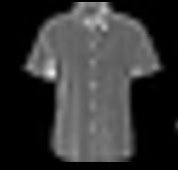
\includegraphics[width=.30\textwidth]{images/shirt.png}};
\node[textonly, right=70pt of shirt] (shirt2) {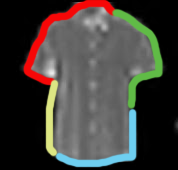
\includegraphics[width=.30\textwidth]{images/shirt2.png}};
\node[textonly, right=60pt of shirt2] (shirt3) {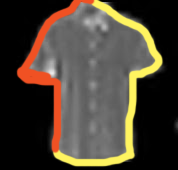
\includegraphics[width=.30\textwidth]{images/shirt3.png}};
\node[textonly, right=60pt of shirt3] (shirt4) {
\includegraphics[width=.30\textwidth]{images/shirt4.png}};


% hidden layer1
\node[op,  right=140pt of x5] (v1) {};
\node[opintense, below=2.5pt of v1] (v2) {};
\node[opintense, below=2.5pt of v2] (v3) {};
\node[op, below=2.5pt of v3] (v4) {};
\node[op, below=2.5pt of v4] (v5) {};
\node[opintense, below=2.5pt of v5] (v6) {};
\node[opintense, below=2.5pt of v6] (v7) {};
\node[op, below=2.5pt of v7] (v8) {};
\node[op, below=2.5pt of v8] (v9) {};


% hidden layer2
\node[op,  right=130pt of v4] (h2) {};
\node[opintense, below=2.5pt of h2] (h3) {};
\node[op, below=2.5pt of h3] (h4) {};
\node[op, above=2.5pt of h2] (h1) {};
\node[opintense, below=2.5pt of h4] (h5) {};


% output layer
\node[op,  right=150pt of h2] (z1) {};
\node[op,  right=150pt of h3] (z2) {};
\node[opintense,  right=150pt of h4] (z3) {};

\node[op,  right=50pt of z1] (y1) {};
\node[op,  right=50pt of z2] (y2) {};
\node[opintense,  below=2.5pt of y2] (y3) {};

%labels

\node[boxtextonly, right=10pt of y1] (lb1) {\huge meia};
\node[boxtextonly, right=10pt of y2] (lb2) {\huge shorts};
\node[boxtextonly, right=10pt of y3] (lb3) {\huge camiseta};




% edges input layer to hidden 1
\path[tedge] (x1) -- (v1);
\path[tedge] (x1) -- (v2);
\path[tedge] (x1) -- (v3);
\path[tedge] (x1) -- (v4);
\path[tedge] (x1) -- (v5);
\path[tedge] (x1) -- (v6);
\path[tedge] (x1) -- (v7);
\path[tedge] (x1) -- (v8);
\path[tedge] (x1) -- (v9);


\path[tedge] (x2) -- (v1);
\path[tedge] (x2) -- (v2);
\path[tedge] (x2) -- (v3);
\path[tedge] (x2) -- (v4);
\path[tedge] (x2) -- (v5);
\path[tedge] (x2) -- (v6);
\path[tedge] (x2) -- (v7);
\path[tedge] (x2) -- (v8);
\path[tedge] (x2) -- (v9);


\path[tedge] (x3) -- (v1);
\path[tedge] (x3) -- (v2);
\path[tedge] (x3) -- (v3);
\path[tedge] (x3) -- (v4);
\path[tedge] (x3) -- (v5);
\path[tedge] (x3) -- (v6);
\path[tedge] (x3) -- (v7);
\path[tedge] (x3) -- (v8);
\path[tedge] (x3) -- (v9);


\path[tedge] (x4) -- (v1);
\path[tedge] (x4) -- (v2);
\path[tedge] (x4) -- (v3);
\path[tedge] (x4) -- (v4);
\path[tedge] (x4) -- (v5);
\path[tedge] (x4) -- (v6);
\path[tedge] (x4) -- (v7);
\path[tedge] (x4) -- (v8);
\path[tedge] (x4) -- (v9);


\path[tedge] (x5) -- (v1);
\path[tedge] (x5) -- (v2);
\path[tedge] (x5) -- (v3);
\path[tedge] (x5) -- (v4);
\path[tedge] (x5) -- (v5);
\path[tedge] (x5) -- (v6);
\path[tedge] (x5) -- (v7);
\path[tedge] (x5) -- (v8);
\path[tedge] (x5) -- (v9);


\path[tedge] (x6) -- (v1);
\path[tedge] (x6) -- (v2);
\path[tedge] (x6) -- (v3);
\path[tedge] (x6) -- (v4);
\path[tedge] (x6) -- (v5);
\path[tedge] (x6) -- (v6);
\path[tedge] (x6) -- (v7);
\path[tedge] (x6) -- (v8);
\path[tedge] (x6) -- (v9);


\path[tedge] (x7) -- (v1);
\path[tedge] (x7) -- (v2);
\path[tedge] (x7) -- (v3);
\path[tedge] (x7) -- (v4);
\path[tedge] (x7) -- (v5);
\path[tedge] (x7) -- (v6);
\path[tedge] (x7) -- (v7);
\path[tedge] (x7) -- (v8);
\path[tedge] (x7) -- (v9);


\path[tedge] (x8) -- (v1);
\path[tedge] (x8) -- (v2);
\path[tedge] (x8) -- (v3);
\path[tedge] (x8) -- (v4);
\path[tedge] (x8) -- (v5);
\path[tedge] (x8) -- (v6);
\path[tedge] (x8) -- (v7);
\path[tedge] (x8) -- (v8);
\path[tedge] (x8) -- (v9);


\path[tedge] (x9) -- (v1);
\path[tedge] (x9) -- (v2);
\path[tedge] (x9) -- (v3);
\path[tedge] (x9) -- (v4);
\path[tedge] (x9) -- (v5);
\path[tedge] (x9) -- (v6);
\path[tedge] (x9) -- (v7);
\path[tedge] (x9) -- (v8);
\path[tedge] (x9) -- (v9);


\path[tedge] (x10) -- (v1);
\path[tedge] (x10) -- (v2);
\path[tedge] (x10) -- (v3);
\path[tedge] (x10) -- (v4);
\path[tedge] (x10) -- (v5);
\path[tedge] (x10) -- (v6);
\path[tedge] (x10) -- (v7);
\path[tedge] (x10) -- (v8);
\path[tedge] (x10) -- (v9);


\path[tedge] (x12) -- (v1);
\path[tedge] (x12) -- (v2);
\path[tedge] (x12) -- (v3);
\path[tedge] (x12) -- (v4);
\path[tedge] (x12) -- (v5);
\path[tedge] (x12) -- (v6);
\path[tedge] (x12) -- (v7);
\path[tedge] (x12) -- (v8);
\path[tedge] (x12) -- (v9);


\path[tedge] (x13) -- (v1);
\path[tedge] (x13) -- (v2);
\path[tedge] (x13) -- (v3);
\path[tedge] (x13) -- (v4);
\path[tedge] (x13) -- (v5);
\path[tedge] (x13) -- (v6);
\path[tedge] (x13) -- (v7);
\path[tedge] (x13) -- (v8);
\path[tedge] (x13) -- (v9);


\path[tedge] (x14) -- (v1);
\path[tedge] (x14) -- (v2);
\path[tedge] (x14) -- (v3);
\path[tedge] (x14) -- (v4);
\path[tedge] (x14) -- (v5);
\path[tedge] (x14) -- (v6);
\path[tedge] (x14) -- (v7);
\path[tedge] (x14) -- (v8);
\path[tedge] (x14) -- (v9);


\path[tedge] (x15) -- (v1);
\path[tedge] (x15) -- (v2);
\path[tedge] (x15) -- (v3);
\path[tedge] (x15) -- (v4);
\path[tedge] (x15) -- (v5);
\path[tedge] (x15) -- (v6);
\path[tedge] (x15) -- (v7);
\path[tedge] (x15) -- (v8);
\path[tedge] (x15) -- (v9);


\path[tedge] (x16) -- (v1);
\path[tedge] (x16) -- (v2);
\path[tedge] (x16) -- (v3);
\path[tedge] (x16) -- (v4);
\path[tedge] (x16) -- (v5);
\path[tedge] (x16) -- (v6);
\path[tedge] (x16) -- (v7);
\path[tedge] (x16) -- (v8);
\path[tedge] (x16) -- (v9);

% edges hiden 1 to hidden 2

\path[tedge] (v1) -- (h1);
\path[tedge] (v1) -- (h2);
\path[tedge] (v1) -- (h3);
\path[tedge] (v1) -- (h4);
\path[tedge] (v1) -- (h5);

\path[tedge] (v2) -- (h1);
\path[tedge] (v2) -- (h2);
\path[tedge] (v2) -- (h3);
\path[tedge] (v2) -- (h4);
\path[tedge] (v2) -- (h5);

\path[tedge] (v3) -- (h1);
\path[tedge] (v3) -- (h2);
\path[tedge] (v3) -- (h3);
\path[tedge] (v3) -- (h4);
\path[tedge] (v3) -- (h5);

\path[tedge] (v4) -- (h1);
\path[tedge] (v4) -- (h2);
\path[tedge] (v4) -- (h3);
\path[tedge] (v4) -- (h4);
\path[tedge] (v4) -- (h5);

\path[tedge] (v5) -- (h1);
\path[tedge] (v5) -- (h2);
\path[tedge] (v5) -- (h3);
\path[tedge] (v5) -- (h4);
\path[tedge] (v5) -- (h5);

\path[tedge] (v6) -- (h1);
\path[tedge] (v6) -- (h2);
\path[tedge] (v6) -- (h3);
\path[tedge] (v6) -- (h4);
\path[tedge] (v6) -- (h5);

\path[tedge] (v7) -- (h1);
\path[tedge] (v7) -- (h2);
\path[tedge] (v7) -- (h3);
\path[tedge] (v7) -- (h4);
\path[tedge] (v7) -- (h5);

\path[tedge] (v8) -- (h1);
\path[tedge] (v8) -- (h2);
\path[tedge] (v8) -- (h3);
\path[tedge] (v8) -- (h4);
\path[tedge] (v8) -- (h5);

\path[tedge] (v9) -- (h1);
\path[tedge] (v9) -- (h2);
\path[tedge] (v9) -- (h3);
\path[tedge] (v9) -- (h4);
\path[tedge] (v9) -- (h5);


% edges hidden to output
\path[tedge] (h1) -- (z1);
\path[tedge] (h1) -- (z2);
\path[tedge] (h1) -- (z3);

\path[tedge] (h2) -- (z1);
\path[tedge] (h2) -- (z2);
\path[tedge] (h2) -- (z3);

\path[tedge] (h3) -- (z1);
\path[tedge] (h3) -- (z2);
\path[tedge] (h3) -- (z3);

\path[tedge] (h4) -- (z1);
\path[tedge] (h4) -- (z2);
\path[tedge] (h4) -- (z3);

\path[tedge] (h5) -- (z1);
\path[tedge] (h5) -- (z2);
\path[tedge] (h5) -- (z3);

% edges output to output
\path[tedge] (z1) edge node[above=1pt] {}  (y1) ;
\path[tedge] (z2) edge node[above=1pt] {}  (y2) ;
\path[tedge] (z3) edge node[above=1pt] {}  (y3) ;




\end{tikzpicture}
} % scalebox
\end{figure}
\end{frame}

\begin{frame}[fragile]{Feedforward neural network  (rede neural)}
\begin{figure}[ht!]
\centering

\scalebox{0.9}{
\begin{tikzpicture}[auto]

% operations =============================

% input layer
\node[op] (x3) {$x_3$};
\node[op, above=10.5pt of x3] (x2) {$x_2$};
\node[op, above=10.5pt of x2] (x1) {$x_1$};
\node[op, below=10.5pt of x3] (x4) {$x_4$};

% hidden layer
\node[state,  above right= 10pt and 90pt of x3] (h2) {$h_2$};
\node[state, below=10.5pt of h2] (h3) {$h_3$};
\node[state, above=10.5pt of h2] (h1) {$h_1$};

% output layer
\node[output,  right=190pt of x3] (out3) {$\hat{y}_3$};
\node[output,  right=190pt of x1] (out1) {$\hat{y}_1$};
\node[output,  right=190pt of x2] (out2) {$\hat{y}_2$};
\node[output,  right=190pt of x4] (out4) {$\hat{y}_4$};


% text only
\node[boxtextonly, above=6.5pt of x1] (entrada) {entrada\\ (\textit{input layer})};
\node[boxtextonly, above=6.5pt of h1] (escondida) {camada escondida\\ (\textit{hidden layer})};
\node[boxtextonly, above=6.5pt of out1] (saida) {sáida\\ (\textit{output layer})};

%edges input to hidden

\path[tedge, line width=1.2mm] (x1) -- (h1);
\path[tedge] (x1) -- (h2);
\path[tedge] (x1) -- (h3);

\path[tedge] (x2) -- (h1);
\path[tedge] (x2) -- (h2);
\path[tedge, line width=1.2mm] (x2) -- (h3);

\path[tedge] (x3) -- (h1);
\path[tedge, line width=1.2mm] (x3) -- (h2);
\path[tedge] (x3) -- (h3);

\path[tedge] (x4) -- (h1);
\path[tedge, line width=1.2mm] (x4) -- (h2);
\path[tedge] (x4) -- (h3);

% edges hidden to output
\path[tedge] (h1) -- (out1);
\path[tedge] (h1) -- (out2);
\path[tedge,line width=1.2mm] (h1) -- (out3);
\path[tedge] (h1) -- (out4);

\path[tedge] (h2) -- (out1);
\path[tedge,line width=1.2mm] (h2) -- (out2);
\path[tedge] (h2) -- (out3);
\path[tedge] (h2) -- (out4);

\path[tedge,line width=1.2mm] (h3) -- (out1);
\path[tedge] (h3) -- (out2);
\path[tedge] (h3) -- (out3);
\path[tedge,line width=1.2mm] (h3) -- (out4);





\end{tikzpicture}
} % scalebox
\end{figure}

\end{frame}

\begin{frame}[fragile]{Versão resumida de uma rede neural}
\begin{figure}[ht!]
\centering

\scalebox{1.5}{
\begin{tikzpicture}[auto]

% operations =============================
\node[state] (h) {$\vect{h}$};
\node[output, above=30pt of h] (y) {$\hat{\vect{y}}$};
\node[op, below=30pt of h] (x) {$\vect{x}$};


% edges
\path[tedge] (x) -- (h);
\path[tedge] (h) -- (y);

\end{tikzpicture}
} % scalebox
\end{figure}

\end{frame}

\begin{frame}{Treinamento}
\begin{figure}[ht!]
\centering

\scalebox{0.8}{
\begin{tikzpicture}[auto]

% nodes =============================
\node[box] (ent) {entrada};
\node[box, right=40pt of ent] (NN) {modelo};
\node[box, right=40pt of NN] (saida) {saída};
\node[textonly, right=18pt of saida] (inv1) {};
\node[textonly, below=5pt of inv1] (inv2) {};
\node[box, right=40pt of saida] (saidaesp) {saída \\ esperada};
\node[boxtextonly, below=90pt of inv1] (comp) {Comparação \\ Erro};
\node[boxtextonly, left=70pt of comp] (Uso) {Alteração \\ dos \\ parâmetros};

% edges =============================
\path[tedge, orange!120, line width=1mm] (ent) -- (NN);
\path[tedge, orange!120, line width=1mm] (NN) -- (saida);
\path[tedge, orange!120, line width=0.5mm] (saida) -- (saidaesp);
\path[tedge, orange!120, line width=0.5mm] (saidaesp) -- (saida);
\path[tedge, orange!120, line width=1mm] (inv2) -- (comp);
\path[tedge, orange!120, line width=1mm] (comp) -- (Uso);
\path[tedge, orange!120, line width=1mm] (Uso) -- (NN);


% animation ============================

\visible<2->{\node[textonly, above=5pt of ent] (shirt) {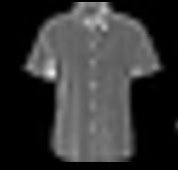
\includegraphics[width=.10\textwidth]{images/shirt.png}};}

\visible<3->{\node[textonly, above=8pt of NN] (rede) {Rede Neural};}

\visible<4->{\node[textonly, above=8pt of saida] (saida2) {meia};}

\visible<5->{\node[textonly, above=8pt of saidaesp] (saida3) {camisa};}

\visible<6->{\node[textonly, below=15pt of comp] (ce) {Entropia cruzada};}

\visible<7->{\node[boxtextonly, left=15pt of Uso] (sgd) {Descida \\do \\Gradiente};}

\end{tikzpicture}
} % scalebox
\end{figure}

\end{frame}


\begin{frame}[fragile]{Descida do gradiente}
\begin{figure}
\centering
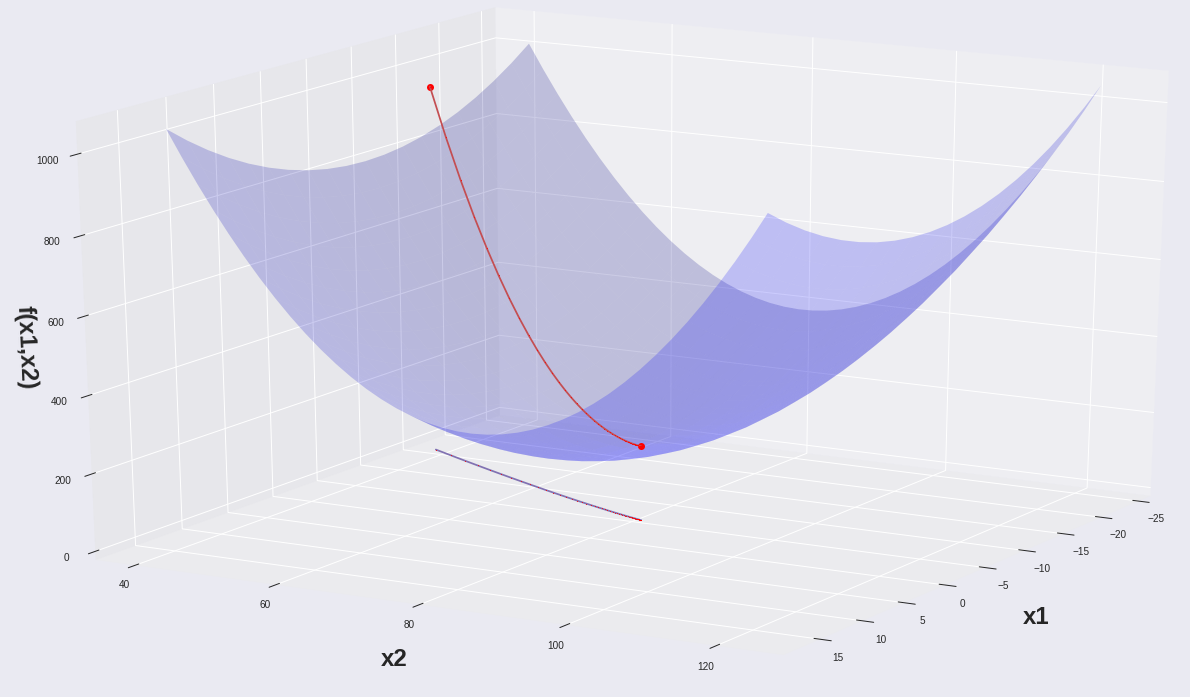
\includegraphics[width=1.0\linewidth]{images/Minimization_image.png}
\end{figure}
\end{frame}

\section{Aprendizado de máquina em linguística}

\begin{frame}[fragile]{On Learning the Past Tenses of English Verbs}

Problema:
\begin{itemize}
\item Aprendizado dos verbos "irregulares" no passado do inglês
\vspace{0.2cm}
\visible<2->{\item Famílias de verbos irregulares:}
\vspace{0.1cm}
	\visible<3->{\begin{itemize}
	\item “blow–blew, grow–grew, know–knew, throw–threw”
	\item “bind–bound, find–found, grind–ground, wind–wound”
	\item “drink–drank, shrink–shrank, sink–sank, stink–stank”}
	\end{itemize}
\vspace{0.2cm}
\visible<4->{\item Chomsky vs Rumelhart e McClelland}
\vspace{0.2cm}
\visible<5->{\item \alert{Regras} (Racionalismo) vs  \alert{Analogias} (Conexionismo)}
\end{itemize}

\end{frame}


\begin{frame}[fragile]{On Learning the Past Tenses of English Verbs}

Exemplo de entrada $\vect{x}$ e saída $\vect{y}$:

\begin{itemize}
\item [] $(\vect{x}^{(1)}, \vect{y}^{(1)}) =$ (begin, began).
\item [] $(\vect{x}^{(2)}, \vect{y}^{(2)}) =$ (love, loved)
\item [] $(\vect{x}^{(3)}, \vect{y}^{(3)}) =$ (drink, drank)
\item [] $(\vect{x}^{(4)}, \vect{y}^{(4)}) =$ (hate, hated)
\item [] $(\vect{x}^{(5)}, \vect{y}^{(5)}) =$ (grow, grew)
\item [] $(\vect{x}^{(6)}, \vect{y}^{(6)}) =$ (bind, bound)
\item [] $(\vect{x}^{(7)}, \vect{y}^{(7)}) =$ (hit, hit)
\item [] $\dots$
\end{itemize}
\end{frame}


\begin{frame}[fragile]{On Learning the Past Tenses of English Verbs}

$\vect{x}$ será uma combinação de traços (features) fonológicos.

\begin{table}[]
\centering
\caption{Categorização de Fonemas em 4 dimensões simples}
\label{fontable}
\begin{tabular}{llllllll}
\hline
 &  & \multicolumn{6}{c}{Place} \\ \hline
 &  & \multicolumn{2}{c|}{Front} & \multicolumn{2}{c|}{Middle} & \multicolumn{2}{c}{Back} \\ \hline
 &  & \multicolumn{1}{l|}{V/L} & \multicolumn{1}{l|}{U/S} & \multicolumn{1}{l|}{V/L} & \multicolumn{1}{l|}{U/S} & \multicolumn{1}{l|}{V/L} & U/S \\ \hline
 \multicolumn{1}{c}{\multirow{2}{*}{Int.}} & Stop & b & p & d & t & g & k \\ \cline{2-8} 
\multicolumn{1}{c}{} & Nasal & m & - & n & - & N & - \\ \hline
\multirow{2}{*}{Cont} & Fric & v/D & f/T & z & s & Z/j & S/C \\ \cline{2-8} 
 & Liq/SV & w/l & - & r & - & y & h \\ \hline
 \multirow{2}{*}{Vowel} & High & E & i & O & - & U & u \\ \cline{2-8} 
 & Low & A & e & I & a/$\alpha$ & W & o \\ \hline
\end{tabular}
\end{table}

\end{frame}

\begin{frame}[fragile]{Explicando as features}
Exemplo: begin
\vspace{1cm}
\\
\begin{tikzpicture}[auto]
%image
\node[textonly] (b) {b};
\node[textonly, right = 30pt of b] (stop) {stop};
\node[textonly, above = 10pt of stop] (int) {int};
\node[textonly, below = 10pt of stop] (front) {front};
\node[textonly, below = 10pt of front] (voiced) {voiced};

\node[textonly, right = 30pt of stop] (e) {e};
\node[textonly, right = 30pt of e] (vowel) {vowel};
\node[textonly, above = 10pt of vowel] (low) {low};
\node[textonly, below = 10pt of vowel] (front1) {front};
\node[textonly, below = 10pt of front1] (short) {short};

\node[textonly, right = 30pt of vowel] (g) {g};
\node[textonly, right = 30pt of g] (int1) {int};
\node[textonly, above = 10pt of int1] (stop1) {stop};
\node[textonly, below = 10pt of int1] (back) {back};
\node[textonly, below = 10pt of back] (voiced1) {voiced};


%paths
\path[tedge] (b) -- (int);
\path[tedge] (b) -- (stop);
\path[tedge] (b) -- (front);
\path[tedge] (b) -- (voiced);

\path[tedge] (e) -- (low);
\path[tedge] (e) -- (vowel);
\path[tedge] (e) -- (front1);
\path[tedge] (e) -- (short);

\path[tedge] (g) -- (int1);
\path[tedge] (g) -- (stop1);
\path[tedge] (g) -- (back);
\path[tedge] (g) -- (voiced1);


\end{tikzpicture}

\end{frame}

\begin{frame}[fragile]{Wickelfeatures}

Wickelfeatures: Trigramas de features
\vspace{0.4cm}
\\Exemplo: begin
\begin{figure}[ht!]
\centering

\scalebox{1.12}{
\begin{tikzpicture}[auto]

\node (beg) {bEg};
\node[right=2.4cm of beg] (egi) {Egi};
\node[right=2.4cm of egi] (gin) {giN};

\visible<2->{\node[below = 0.2cm of beg] (fbeg){$\footnotesize{\begin{bmatrix} int,high,int\\int, vowel,int\\int,front,int\\int,long,int\\stop,high,stop\\stop,vowel,stop\\stop,front,stop\\stop,long,stop\\\vdots\\voiced,front,voiced\\voiced,long,voiced\end{bmatrix}}$};};

 \visible<3->{\node[below = 0.2cm of egi] (fegi){$\footnotesize{\begin{bmatrix} vowel,int,vowel\\vowel,stop,vowel\\vowel,back,vowel\\vowel,voiced,vowel\\high,int,high\\high,stop,high\\high,back,high\\high,voiced,high\\\vdots\\short,int,short\\short,voiced,short\end{bmatrix}}$};
\node[below = 0.2cm of gin] (gin){$\footnotesize{\begin{bmatrix} int,vowel,int\\int,high,int\\int,front,int\\int,short,int\\stop,vowel,nasal\\stop,high,nasal\\stop,front,nasal\\stop,short,nasal\\\vdots\\back,vowel,back\\back,high,back\end{bmatrix}}$};};


\end{tikzpicture}
} % scalebox
\end{figure}
\end{frame}



\begin{frame}[fragile]{On Learning the Past Tenses of English Verbs}
\begin{figure}[ht!]
\centering

\scalebox{1.15}{
\begin{tikzpicture}[auto]

\node[textonly] (xlabel) {$\vect{x} \, \, \, \,=$};
\node[textonly, right=2pt of xlabel] (xvalue) {$\begin{bmatrix} 1\\0\\0\\\vdots\\1\\0\\\vdots\\0\end{bmatrix}$};

\node[textonly] at (3,1.93)  (phon1) {int, vowel, int};
\node[textonly, below=0.5pt of phon1]  (phon2) {int, vowel, cont};
\node[textonly, below=0.5pt of phon2]  (phon3) {bla, bla, bla};
\node[textonly, below=0.5pt of phon3]  (phon4) {};
\node[textonly, below=5pt of phon4]  (phon5) {bla, bla, bla};
\node[textonly, below=0.5pt of phon5]  (phon6) {bla, bla, bla};
\node[textonly, below=0.5pt of phon6]  (phon7) {};
\node[textonly, below=0.5pt of phon7]  (phon8) {};
\node[textonly, below=5pt of phon8]  (phon9) {bla, bla, bla};


\end{tikzpicture}
} % scalebox
\end{figure}


\end{frame}


\begin{frame}[fragile]{On Learning the Past Tenses of English Verbs}
\begin{figure}[ht!]
\centering

\scalebox{1.15}{
\begin{tikzpicture}[auto]

\node[textonly] (xlabel) {$\vect{\hat{y}} \, \, \, \,=$};
\node[textonly, right=2pt of xlabel] (xvalue) {$\begin{bmatrix} 0.234\\0.967\\0.123\\\vdots\\0.152\\0.876\\\vdots\\0.765\end{bmatrix}$};

\node[textonly] at (5,1.93)  (phon1) {int, vowel, int};
\node[textonly, below=0.5pt of phon1]  (phon2) {int, vowel, cont};
\node[textonly, below=0.5pt of phon2]  (phon3) {int, vowel, vowel};
\node[textonly, below=0.5pt of phon3]  (phon4) {};
\node[textonly, below=5pt of phon4]  (phon5) {low, int, high};
\node[textonly, below=0.5pt of phon5]  (phon6) {low, int, low};
\node[textonly, below=0.5pt of phon6]  (phon7) {};
\node[textonly, below=0.5pt of phon7]  (phon8) {};
\node[textonly, below=5pt of phon8]  (phon9) {short, voiced, short};


\end{tikzpicture}
} % scalebox
\end{figure}

\end{frame}

\begin{frame}[fragile]{On Learning the Past Tenses of English Verbs}
\begin{figure}[ht!]
\centering

\scalebox{1.15}{
\begin{tikzpicture}[auto]

\node[textonly] (predlabel) {$\vect{\hat{y}} \, \, \, \,=$};
\node[textonly, right=2pt of predlabel] (predvalue) {$\begin{bmatrix} 0.234\\0.967\\0.123\\\vdots\\0.152\\0.876\\\vdots\\0.765\end{bmatrix}$};

\node[textonly, right=12pt of predvalue] (yvalue) {$\begin{bmatrix} 1\\1\\0\\\vdots\\0\\1\\\vdots\\1\end{bmatrix}$};
\node[textonly, right=2pt of yvalue] (ylabel) {$= \, \, \, \,\vect{y}$};

\node[textonly, below left=-13pt and -5pt of predvalue] (inv1) {};
\node[textonly, below right=-13pt and -5pt of yvalue] (inv2) {};


\node[boxtextonly, below right=30pt and -5pt of inv1] (MSE) {$(\vect{\hat{y}} - \vect{y})^2$\\ erro quadrado médio};



% edges
\draw[orange!120, line width=1mm]  (MSE) to [out=90,in=-90] (inv1);
\draw[orange!120, line width=1mm] (MSE) to [out=90,in=-90] (inv2);



\end{tikzpicture}
} % scalebox
\end{figure}

\end{frame}


\begin{frame}[fragile]{On Learning the Past Tenses of English Verbs}
Resultados (PROS):

\begin{itemize}
\visible<2->{\item Identificou padrões corretamente entre todos os 420 verbos do treinamento;}
\vspace{0.4cm}
\visible<3->{\item Taxa de acerto de 92\% para verbos regulares ausentes no treinamento;}
\vspace{0.4cm}
\visible<4->{\item Taxa de acerto de 84\% para verbos irregulares ausentes no treinamento;}
\vspace{0.4cm}
\visible<5->{\item U-shaped Development}
\end{itemize}
\end{frame}

\begin{frame}[fragile]{On Learning the Past Tenses of English Verbs}
Resultados (CONS):

\begin{itemize}
\visible<2->{\item Falha ao tentar fazer predições com palavras que compartilham muitas features em comum; \\Exemplo: "algalgal" - Oykangand}
\vspace{0.4cm}
\visible<3->{\item Problemas como uma teoria da mente}
\end{itemize}
\end{frame}



\begin{frame}[fragile]{As Irregularidades no Português Brasileiro}
Desafios:
\begin{itemize}
\visible<2->{\item "Wug Test"; \\ Exemplos: "poguir", "redir", "atover"}
\vspace{0.2cm}
\visible<3->{\item Adaptar a rede para a língua portuguesa}
\vspace{0.2cm}
\visible<4->{\item Melhorar o desempenho da rede}
\end{itemize}
\end{frame}

\section{Modelos de linguagem e redes recorrentes}


\begin{frame}{Definition}
Nos chamamos de \alert{modelo de linguagem} uma distribuição de probabildiade sobre uma sequencia de tokens em uma lingua natural.

\[
P(x_1,x_2,x_3,x_4) = p
\]

\textbf{Usamos esse modelo em}:
\begin{itemize}
\item reconhecimento de fala
\item tradução automática
\item text auto-completion
\item correção de texto
\item resposta automatizada
\item sumarização
\end{itemize}


\end{frame}

\begin{frame}{Revisão de probabilidade}
\large{
\begin{itemize}
\item \textbf{Probabilidade condicional} 
\[
P(A|B) = \frac{P(A,B)}{P(B)}
\]
\item \textbf{Independência} 
\[
P(A|B) = P(A)
\]
\item \textbf{Regra da cadeia} 
\[
P(A,B,C) = P(A)P(B|A)P(C|A,B)
\]
\end{itemize}
}
\end{frame}


\begin{frame}{Como calculamos essas probabilidades?}
Regra da cadeia:

\begin{equation*}
P(x_1,x_2,x_3,x_4) = P(x_1)P(x_2\vert x_1)P(x_3\vert x_1x_2)P(x_4\vert x_1x_2x_3)
\end{equation*}

\vspace{0.3cm}

Para simplificação fazemos uma \textbf{suposição de Markov}, i.e., para um  $n$ específico assumimos certas independências, assim cada palavra depende apenas das últimas $n-1$ palavras:



\begin{equation*}
P(x_1, \dots, x_T) = \prod_{t=1}^{T} P(x_t \vert x_1, \dots, x_{t-1}) = \prod_{t=1}^{T} P(x_{t} \vert x_{t - (n+1)}, \dots, x_{t-1})
\end{equation*} 

\end{frame}

\begin{frame}{Modelos baseados em estatísticas de $n$-gramas}
A escolha de $n$ leva a modelos diferentes.\\

\textbf{Modelo de unigrama} ($n=1$): 
\begin{equation*}
P_{uni}(x_1, x_2, x_3, x_4) = P(x_1)P(x_2)P(x_3)P(x_4)
\end{equation*}

em que $P(x_i) = count(x_i)$.\\

\textbf{Modelo de bigrama} ($n=2$): 
\begin{equation*}
P_{bi}(x_1,x_2,x_3,x_4) = P(x_1)P(x_2\vert x_1)P(x_3\vert x_2)P(x_4\vert x_3)
\end{equation*} 
em que
\[
P(x_i\vert x_j) = \frac{count(x_i, x_j)}{count(x_j)}
\]
\end{frame}

\begin{frame}{Estatísticas de $n$-gramas}
\url{https://books.google.com/ngrams}
\vspace{0.4cm}

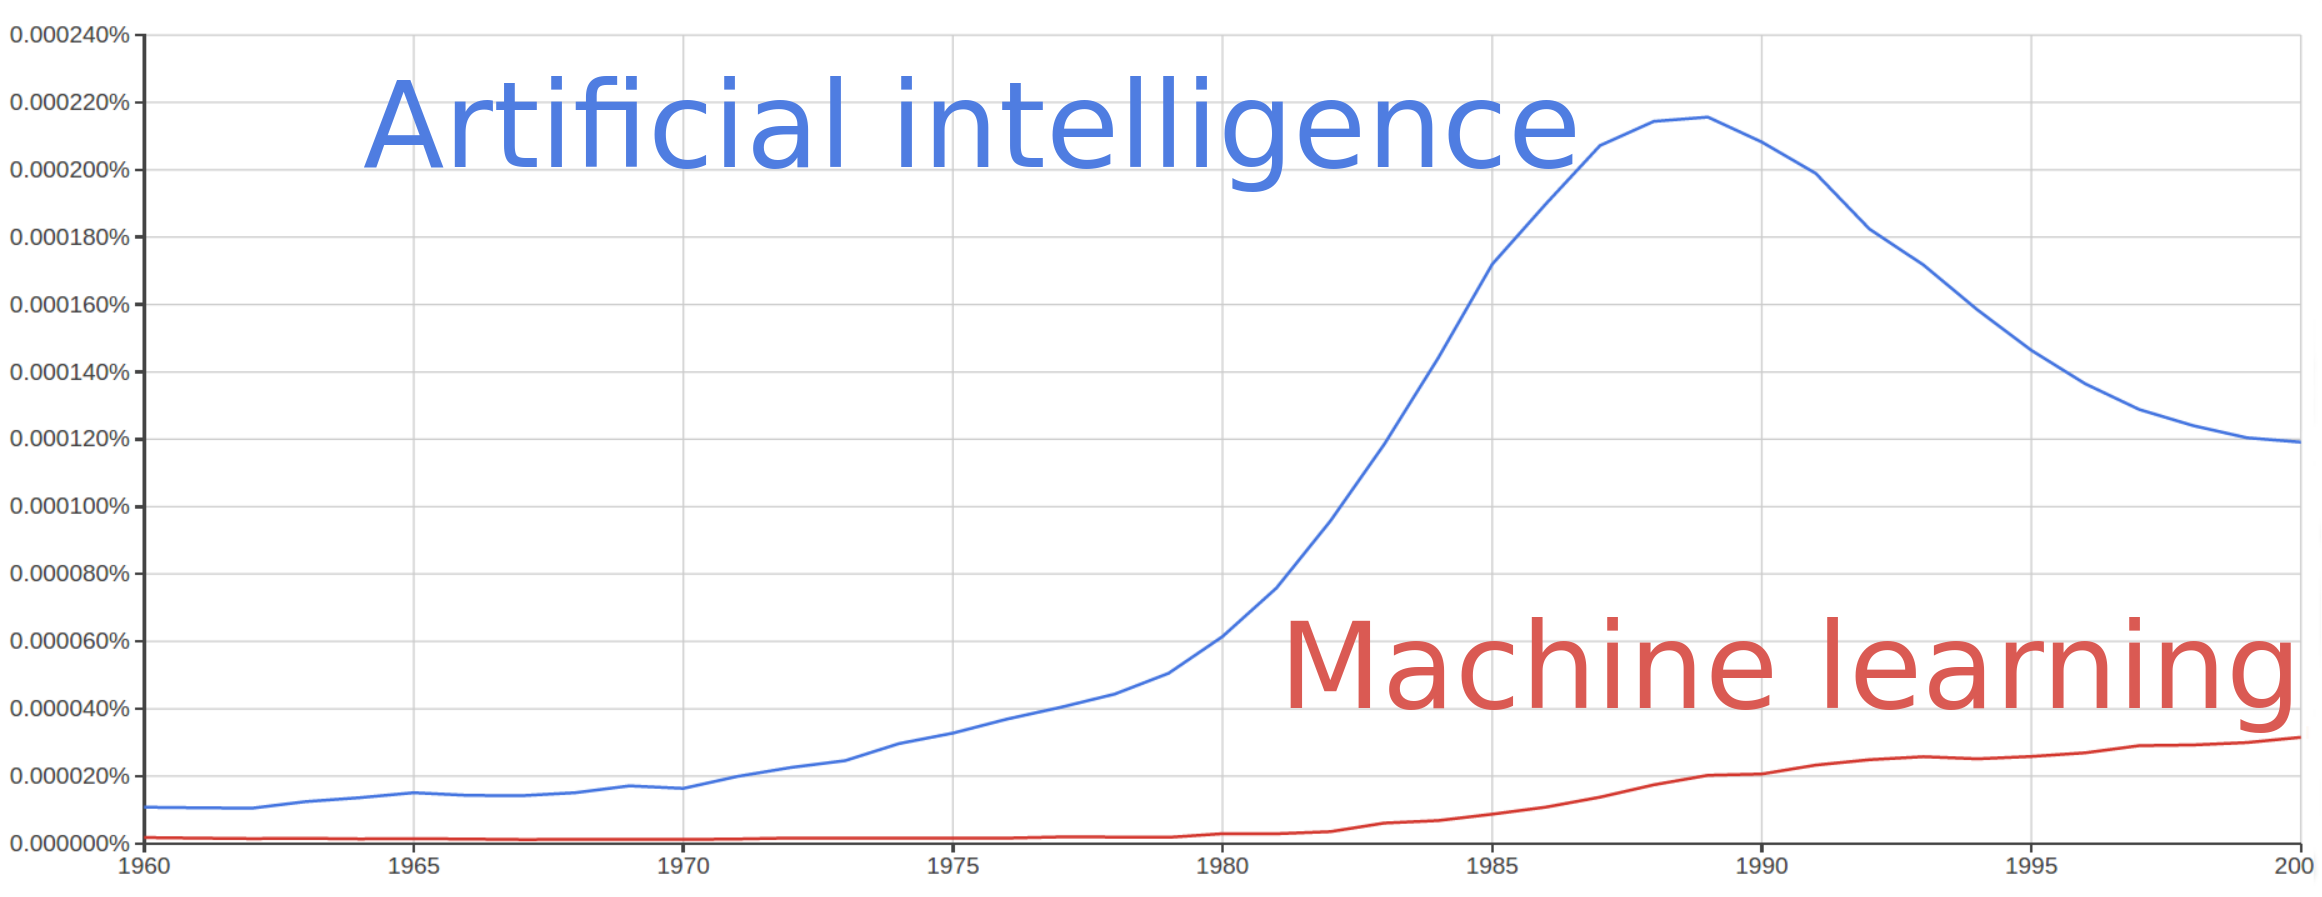
\includegraphics[scale=0.14]{images/AI_ML.png}
\end{frame}



\begin{frame}{Modelos baseados em estatísticas de $n$-gramas}
\begin{itemize}
\item Quanto maior o $n$ melhor a performance do modelo.
\vspace{0.7cm}
\item Quanto maior o $n$ maior o uso de memória!
\vspace{0.1cm}
\begin{quote}
"Using one machine \textbf{with 140 GB
RAM for 2.8 days}, we built an unpruned
model on 126 billion tokens."
\end{quote}
\begin{itemize}
\item [] \textit{Scalable Modified Kneser-Ney Language Model Estimation} by Heafield et al.
\end{itemize}
\end{itemize}
\end{frame}


\begin{frame}{Modelos de linguagem como predição de data sequencial}

Em vez de usar uma abordagem que seja específica para o domínio da linguagem natural, podemos usar um modelo para predição de dados sequencias:  \textbf{uma rede recorrente (RNN)}. \\

Nossa tarefa de aprendizado é estimar a distribuição de probabilidade

\[
P(x_{n} = \text{palavra}_{j^{*}} | x_{1}, \dots ,x_{n-1})
\]

para qualquer $(n-1)$ sequencia de palavras $x_{1}, \dots ,x_{n-1}$.
\end{frame}

\begin{frame}{Classificação com uma deep feedforward network}
\begin{figure}[ht!]
\centering

\scalebox{1.3}{
\begin{tikzpicture}[auto]

% operations =============================

% nodes
\node[textonly] (vectorx) {$\begin{bmatrix}0.34\\ \vdots \\0.06\end{bmatrix}$};
\node[textonly, above=1pt of vectorx] (x) {$\vect{x}$};
\node[textonly, below=1pt of vectorx] (dimension1) {{\small$n\times 1$}};
\node[op, right=30pt of vectorx] (model) {\textbf{DFN}};
\node[textonly, right=30pt of model] (vectoryhat) {$\begin{bmatrix}p(y=1| \vect{x};\vect{\theta})\\ \vdots \\p(y=k| \vect{x};\vect{\theta})\end{bmatrix}$};
\node[textonly, above=1pt of vectoryhat] (yhat) {$\hat{\vect{y}}$};
\node[textonly, below=1pt of vectoryhat] (dimension2) {{\small$k\times 1$}};



% edges
\path[tedge] (vectorx) -- (model);
\path[tedge] (model) -- (vectoryhat);


\end{tikzpicture}
} % scalebox
\end{figure}

\end{frame}

\begin{frame}{Classificação com uma RNN}
\begin{figure}[ht!]
\centering

\scalebox{0.9}{
\begin{tikzpicture}[auto]

% operations =============================

% nodes
\node[textonly] (vectorx1) {$\begin{bmatrix}0.34\\ \vdots \\0.06\end{bmatrix}$};
\node[textonly, above=1pt of vectorx1] (x1) {$\vect{x}^{(1)}$};
\node[textonly, below=15pt of vectorx1] (vectorx2) {$\begin{bmatrix}0.92\\ \vdots \\-0.55\end{bmatrix}$};
\node[textonly, above=1pt of vectorx2] (x2) {$\vect{x}^{(2)}$};
\node[textonly, below=15pt of vectorx2] (vectorx3) {$\begin{bmatrix}-0.53\\ \vdots \\1.1\end{bmatrix}$};
\node[textonly, above=1pt of vectorx3] (x3) {$\vect{x}^{(3)}$};


\node[op, right=30pt of vectorx2] (model) {\textbf{RNN}};
\node[textonly, right=30pt of model] (vectoryhat) {$\begin{bmatrix}p(y=1|\; \vect{x}^{(1)},\vect{x}^{(2)}, \vect{x}^{(3)};\vect{\theta})\\ \vdots \\p(y=k|\; \vect{x}^{(1)},\vect{x}^{(2)}, \vect{x}^{(3)};\vect{\theta})\end{bmatrix}$};
\node[textonly, above=1pt of vectoryhat] (yhat) {$\hat{\vect{y}}$};



% edges
\path[tedge] (vectorx1) -- (model);
\path[tedge] (vectorx2) -- (model);
\path[tedge] (vectorx3) -- (model);
\path[tedge] (model) -- (vectoryhat);


\end{tikzpicture}
} % scalebox
\end{figure}

\end{frame}

\begin{frame}{Classificação com uma RNN}
\begin{figure}[ht!]
\centering

\scalebox{0.85}{
\begin{tikzpicture}[auto]

% operations =============================

% nodes
\node[textonly] (vectorx1) {$\begin{bmatrix}0.34\\ \vdots \\0.06\end{bmatrix}$};
\node[textonly, above=1pt of vectorx1] (x1) {$\vect{x}^{(1)}$};
\node[textonly, below=15pt of vectorx1] (vectorx2) {$\begin{bmatrix}0.92\\ \vdots \\-0.55\end{bmatrix}$};
\node[textonly, above=1pt of vectorx2] (x2) {$\vect{x}^{(2)}$};
\node[textonly, below=15pt of vectorx2] (vectorx3) {$\begin{bmatrix}-0.53\\ \vdots \\1.1\end{bmatrix}$};
\node[textonly, above=1pt of vectorx3] (x3) {$\vect{x}^{(3)}$};


\node[op, right=30pt of vectorx2] (model) {\textbf{RNN}};
\node[textonly, right=30pt of model] (vectoryhat) {$\begin{bmatrix}p(y=\text{positivo}|\; \vect{x}^{(1)},\vect{x}^{(2)}, \vect{x}^{(3)};\vect{\theta})\\p(y=\text{neutro}|\; \vect{x}^{(1)},\vect{x}^{(2)}, \vect{x}^{(3)};\vect{\theta}) \\p(y=\text{negativo}|\; \vect{x}^{(1)},\vect{x}^{(2)}, \vect{x}^{(3)};\vect{\theta})\end{bmatrix}$};
\node[textonly, above=1pt of vectoryhat] (yhat) {$\hat{\vect{y}}$};


\visible<2->{\node[textonly, below=12pt of vectoryhat] (xslabels) {$\vect{x}^{(1)} \; \; \; \; \vect{x}^{(2)} \; \; \; \; \vect{x}^{(3)}$};}
\visible<2->{\node[textonly, below=-2pt of xslabels] (sentence) {Bonito mas idiota};}

\visible<3->{\node[textonly, below=20pt of xslabels] (yslabels) {$\vect{y}^{(1)}, \; \; \; \; \vect{y}^{(2)}, \; \; \; \; \vect{y}^{(3)}$};}
\visible<3->{\node[textonly, below=-2pt of yslabels] (groundtruht) {positivo, neutro, negativo};}

\visible<4->{\node[textonly, right=1pt of vectoryhat] (ys) {$=\begin{bmatrix}0.2\\0.1\\0.7\end{bmatrix}$};}



% edges
\path[tedge] (vectorx1) -- (model);
\path[tedge] (vectorx2) -- (model);
\path[tedge] (vectorx3) -- (model);
\path[tedge] (model) -- (vectoryhat);


\end{tikzpicture}
} % scalebox
\end{figure}

\end{frame}


\begin{frame}[fragile]{RNNs}
\begin{figure}[ht!]
\centering

\scalebox{1.40}{
\begin{tikzpicture}[auto]

% RNN state cell =============================
\node[state] (h) {$\vect{h}$};
\node[op, below=30pt of h] (x) {$\vect{x}$};
\node[output, above=30pt of h] (yhat) {$\hat{\vect{y}}$};



% edges
\path[tedge] (x) edge node[below right= -4pt] {}  (h) ;
\path[tedge] (h) edge [out=-400,in=-320,looseness=8, distance=125pt] node[above right] {} (h);
\path[tedge] (h) edge node[below right = -4pt] {} (yhat);


\end{tikzpicture}
} % scalebox
\end{figure}

\end{frame}


\begin{frame}[fragile]{RNNs}
% RNN STATE CELL ====================================
\newcommand{\rnnSimple}[4]{

% operations
\node[state, minimum size=40pt,#4] (h#3) {$\vect{h}^{#1}$};
\node[op, minimum size=40pt,below=30pt of h#3] (x#3) {$\vect{x}^{#1}$};
\node[output, minimum size=40pt, above=30pt of h#3] (yhat#3) {$\hat{\vect{y}}^{#1}$};

% edges
\path[tedge] (x#3) edge node[below right= -4pt] {} (h#3);
\path[tedge] (h#3) edge node[below right = -4pt] {} (yhat#3);
}

\begin{figure}[ht!]
\hspace*{-1.0cm}
\scalebox{0.9}{
\begin{tikzpicture}[auto]

% timestep 1
\rnnSimple{(1)}{(0)}{t1}{}

% % timestep 0
\node[state, minimum size=40pt,left=50pt of ht1] (ht0) {$\vect{h}^{(0)}$};

% % timestep 2
\rnnSimple{(2)}{(1)}{t2}{right=50pt of ht1};


% % timestep 2
\rnnSimple{(3)}{(1)}{t3}{right=50pt of ht2};


% % state transfers
\path[tedge] (ht0) edge node[above right = 2pt] {} (ht1);
\path[tedge] (ht1) edge node[above right = 2pt] {} (ht2);
\path[tedge] (ht2) edge node[above right = 2pt] {} (ht3);

\end{tikzpicture}
}%\scalebox
\end{figure}


\end{frame}



\begin{frame}{Exemplo de um dataset}
Nos separamos um corpus $C$ com $T$ tokens e vocabulário $\Vocab$.\\\

Exemplo: \textbf{Make Some Noise}, the Beastie Boys.\\

\begin{quote}
\alert{Yes, here we go again, give you more, nothing lesser\\
Back on the mic is the anti-depressor\\
Ad-Rock, the pressure, yes, we need this\\
The best is yet to come, and yes, believe this\\
... \\}
\end{quote}

\begin{itemize}
\item $T = 378$
\item $|\Vocab| = 186$
\end{itemize}

\end{frame}

\begin{frame}{Exemplo de um dataset}
O dataset é uma coleção de pares $(\vect{x},\vect{y})$ em que $\vect{x}$ é uma palavra e $\vect{y}$ é a palavra imediatamente a direita. Por exemplo:
\begin{itemize}
\item [] $(\vect{x}^{(1)}, \vect{y}^{(1)}) =$ (Yes, here).
\item [] $(\vect{x}^{(2)}, \vect{y}^{(2)}) =$ (here, we)
\item [] $(\vect{x}^{(3)}, \vect{y}^{(3)}) =$ (we, go)
\item [] $(\vect{x}^{(4)}, \vect{y}^{(4)}) =$ (go, again)
\item [] $(\vect{x}^{(5)}, \vect{y}^{(5)}) =$ (again, give)
\item [] $(\vect{x}^{(6)}, \vect{y}^{(6)}) =$ (give, you)
\item [] $(\vect{x}^{(7)}, \vect{y}^{(7)}) =$ (you, more)
\item [] $\dots$
\end{itemize}
\end{frame}


\begin{frame}{O modelo de linguagem com RNN}
\begin{figure}[ht!]
\centering

\scalebox{1.40}{
\begin{tikzpicture}[auto]

% RNN state cell =============================
\node[state] (h) {$\vect{h}$};
\node[op, below=30pt of h] (e) {$\vect{e}$};
\node[output, above=30pt of h] (yhat) {$\hat{\vect{y}}$};

\node[textonly, below right=0.5pt and 0.5pt of e] (inv1) {};
\node[textonly, above right=0.5pt and 0.5pt of e] (inv2) {};
\node[textonly, right=40pt of e] (embedding) {camada de embedding};





% edges
\path[tedge] (e) edge node[below right= -4pt] {}  (h) ;
\path[tedge] (h) edge [out=-400,in=-320,looseness=8, distance=125pt] node[above right] {$\vect{W}$} (h);
\path[tedge] (h) edge node[below right = -4pt] {} (yhat);


% % info edges
\draw[orange!120, line width=1mm]  (embedding) to [out=-180,in=0] (inv1);
\draw[orange!120, line width=1mm] (embedding) to [out=-180,in=0] (inv2);


\end{tikzpicture}
} % scalebox
\end{figure}

\end{frame}

\begin{frame}{Word Embeddings}
\begin{figure}[ht!]
\centering

\scalebox{1.35}{
\begin{tikzpicture}[auto]

\node[textonly] (vectorx) {$\begin{bmatrix}0\\ \vdots\\ 1 \\\vdots \\0\end{bmatrix}$};
\node[textonly, above=1pt of vectorx] (x) {$\vect{x}$};
\node[textonly, below=1pt of vectorx] (dimension1) {{\small$|\Vocab|\times 1$}};

\node[textonly, left=50pt of vectorx] (word) {Yes};

\node[textonly, right=50pt of vectorx] (vectore) {$\begin{bmatrix}0.33\\ \vdots\\0.67\end{bmatrix}$};
\node[textonly, above=1pt of vectore] (e) {$\vect{e}$};
\node[textonly, below=1pt of vectore] (dimension2) {{\small$n\times 1$}};

\path[tedge, orange!120, line width=1mm] (word) edge node[above left= 1pt and -15pt] {one hot}  (vectorx);
\path[tedge, orange!120, line width=1mm] (vectorx) edge node[above left= 1pt and -30pt] {embedding}  (vectore);



\end{tikzpicture}
} % scalebox
\end{figure}


\end{frame}


\begin{frame}{O modelo de linguagem com RNN}
% RNN STATE CELL ====================================
\newcommand{\rnnSimple}[4]{

% operations
\node[state, minimum size=40pt,#4] (h#3) {$\vect{h}^{#1}$};
\node[op, minimum size=40pt, above=30pt of h#3] (yhat#3){$\hat{\vect{y}}^{#1}$};
\node[op, minimum size=40pt,below=30pt of h#3] (e#3) {$\vect{e}^{#1}$};
\node[textonly, below=0.1pt of e#3] {{\Large#2}};

% edges
\path[tedge] (e#3) edge node[below right= -4pt] {$\vect{U}$} (h#3);
\path[tedge] (h#3) edge node[below right = -4pt] {$\vect{V}$} (yhat#3);
}

\begin{figure}[ht!]
\hspace*{-1.0cm}
\scalebox{0.8}{
\begin{tikzpicture}[auto]

% timestep 1
\rnnSimple{(1)}{Yes}{t1}{}

% % timestep 0
\node[state, minimum size=40pt,left=50pt of ht1] (ht0) {$\vect{h}^{(0)}$};

% % timestep 2
\rnnSimple{(2)}{here}{t2}{right=50pt of ht1};


% % timestep 2
\rnnSimple{(3)}{we}{t3}{right=50pt of ht2};


% % state transfers
\path[tedge] (ht0) edge node[above right = 2pt] {$\vect{W}$} (ht1);
\path[tedge] (ht1) edge node[above right = 2pt] {$\vect{W}$} (ht2);
\path[tedge] (ht2) edge node[above right = 2pt] {$\vect{W}$} (ht3);

% text
\node[textonly, above=40pt of yhatt2] (result) {{\Large $P(x^{(4)}| \text{Yes, here, we})$}};

% Arrow to result
%  \path[tedge] (yhatt3)  edge node[bend right, out=-50, distance=25pt] (result);
\draw[->, line width=1mm] [bend right, out=-50, distance=25pt](yhatt3.north) to  (result.east);
%  \path[tedge] (yhatt3.north) to [bend right, out=-50, distance=25pt] (result.east);




\end{tikzpicture}
}%\scalebox
\end{figure}


\end{frame}

\begin{frame}{Dificuldades ao se treinar uma RNN}

\begin{itemize}
\item Quando nos inicializamos $\vect{W}$ de modo que $||\vect{W}|| < 1$, os gradientes dos passos mais antigos vão sumir (\alert{vanishing problem}).
\vspace{0.2cm}
\item E quando $||\vect{W}|| > 1$, os gradientes dos passos mais antigos vão explodir (\alert{exploding problem}).
\vspace{0.2cm}
\item Como resultado os gradientes dos passos mais próximos ao passo final vão ter mais influência do que os passos mais distantes. Isso é ruim para capturar \alert{longas dependências}.
\vspace{0.2cm}
\begin{itemize}
\visible<2->{\item[] Eu fui morar na \textbf{frança}, com uma $\_\_\_\_\_\_\_$.} \visible<3->{\textbf{(francesa)}}
\vspace{0.3cm}
\visible<4->{\item[] Eu fui morar na \textbf{frança}, nesse tempo fiquei estudando a língua $\_\_\_\_\_\_\_$.} \visible<5->{\textbf{(francesa)}}
\vspace{0.3cm}
\visible<6->{\item[] Eu fui morar na \textbf{frança} durante três anos e cinco meses com dois amigos, o Carlos e o Lucas. Foi bem legal, nesse tempo fiquei estudando a língua $\_\_\_\_\_\_\_$.} \visible<7->{\textbf{(francesa)}}
\end{itemize}
\end{itemize}
\end{frame}

\begin{frame}{Algumas soluções}
\begin{itemize}
\item GRU (Gated Recurrent Unit)
\vspace{0.2cm}
\item LSTM (Long Short-Term Memory).
\end{itemize}
\vspace{0.2cm}
% RNN STATE CELL ====================================
\newcommand{\rnnSimple}[4]{

% operations
\node[state, minimum size=30pt,#4] (h#3) {$\vect{h}^{#1}$};
\node[state, minimum size=30pt,above left=10pt and 10pt of h#3] (C#3) {$\vect{C}^{#1}$};
\node[textonly, above right=5pt and 5pt of h#3] (inv#3) {};
\node[op, minimum size=40pt,below=30pt of h#3] (x#3) {$\vect{x}^{#1}$};
\node[output, minimum size=40pt, above=50pt of h#3] (yhat#3) {$\hat{\vect{y}}^{#1}$};


%% namedscope LSTM cell
\begin{scope}[on background layer]
\coordinate (p1) at (inv#3.north);
\coordinate (p2) at (h#3.south east);
\coordinate (p3) at (C#3.north west);
\tkzCircumCenter(p1,p2,p3)
\tkzGetPoint{O}
\tkzDrawCircle[draw=orange, line width=1.5pt, fill=orange!60](O,p1)
\end{scope}


% edges
\path[tedge] (x#3) -- (h#3);
\path[tedge] (h#3)-- (yhat#3);
}

\begin{figure}[ht!]
\hspace*{-1.0cm}
\scalebox{0.85}{
\begin{tikzpicture}[auto]

% timestep 1
\rnnSimple{(1)}{(0)}{t1}{}

% % timestep 0
\node[state, minimum size=30pt,left=50pt of ht1] (ht0) {$\vect{h}^{(0)}$};
\node[state, minimum size=30pt,left=17pt of Ct1] (Ct0) {$\vect{C}^{(0)}$};

% % timestep 2
\rnnSimple{(2)}{(1)}{t2}{right=50pt of ht1};


% % timestep 2
\rnnSimple{(3)}{(1)}{t3}{right=50pt of ht2};


% % state transfers
\path[tedge] (ht0) -- (ht1);
\path[tedge] (ht1) -- (ht2);
\path[tedge] (ht2) -- (ht3);
\path[tedge] (Ct0) -- (Ct1);
\path[tedge] (Ct1) -- (Ct2);
\path[tedge] (Ct2) -- (Ct3);



\end{tikzpicture}
}%\scalebox
\end{figure}

\end{frame}

\begin{frame}{Exemplo de aplicação: TrumpBot}
\url{https://github.com/felipessalvatore/MyTwitterBot}
\begin{center}
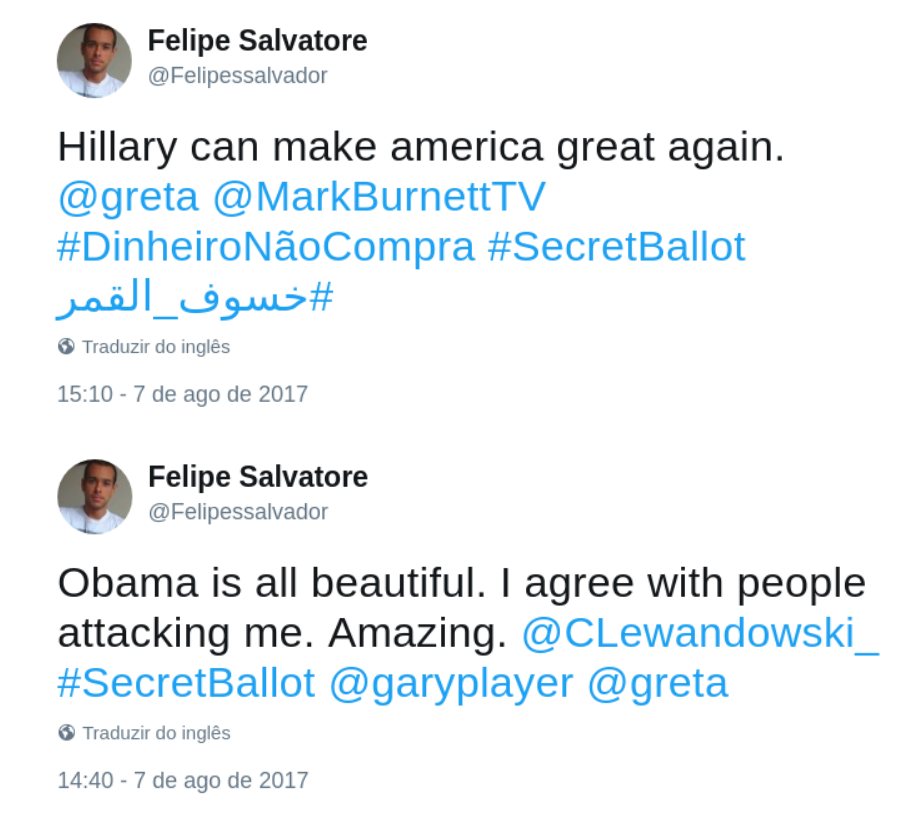
\includegraphics[scale=0.24]{images/TrumpBot.png}
\end{center}
\end{frame}

\begin{frame}{Exemplo de aplicação: SakaBot}
\url{https://github.com/felipessalvatore/MyTwitterBot}
\begin{center}
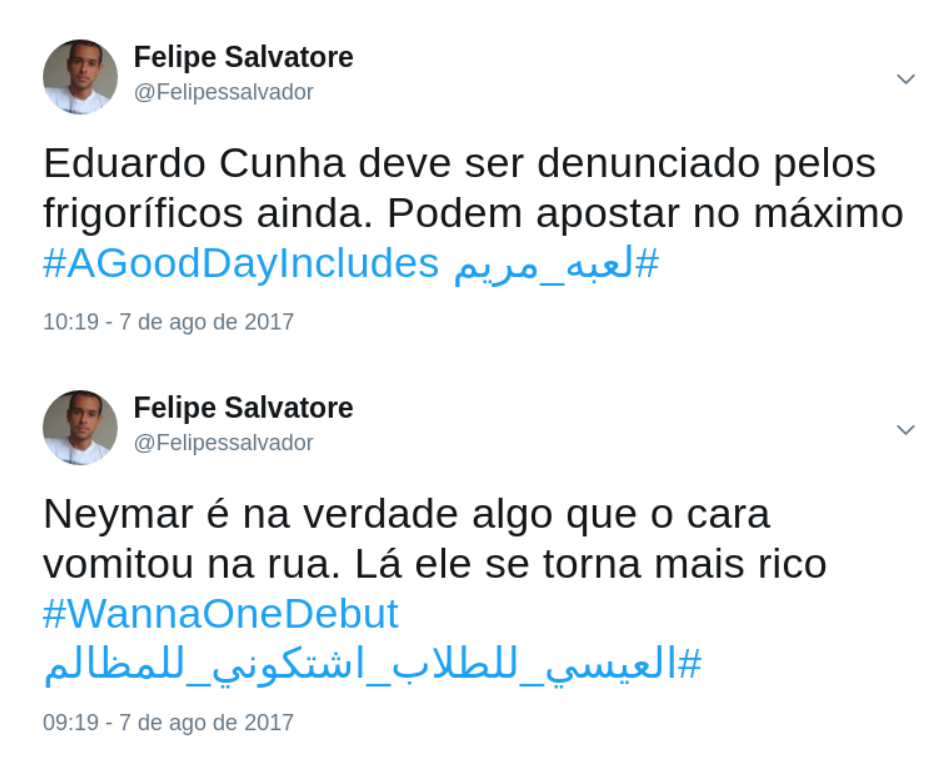
\includegraphics[scale=0.24]{images/SakaBot.png}
\end{center}
\end{frame}


\begin{frame}{Tradução automatica}
% RNN encoder ====================================
\newcommand{\rnnencoder}[4]{

% operations
\node[state, minimum size=40pt,#4] (h#3) {$\vect{h}^{#1}$};
\node[op, minimum size=40pt,below=30pt of h#3] (e#3) {$\vect{e}^{#1}$};
\node[textonly, below=0.1pt of e#3] {{\Large#2}};

% edges
\path[tedge] (e#3) edge node[below right= -4pt] {} (h#3);
}

% RNN decoder ====================================
\newcommand{\rnndecoder}[4]{

% operations
\node[state, minimum size=40pt,#4] (h#3) {${\vect{h}^{\prime}}^{#1}$};
\node[output, minimum size=40pt, above=30pt of h#3] (yhat#3){$\hat{\vect{y}}^{#1}$};
\node[op, minimum size=40pt,below=30pt of h#3] (x#3) {$\vect{x}^{#1}$};
\node[textonly, below=0.1pt of x#3] {{\Large#2}};

% edges
\path[tedge] (x#3) edge node[below right= -4pt] {} (h#3);
\path[tedge] (h#3) edge node[below right = -4pt] {} (yhat#3);
}


\newcommand{\rnndecoderSimpl}[4]{

% operations
\node[state, minimum size=40pt,#4] (h#3) {${\vect{h}^{\prime}}^{#1}$};
\node[op, minimum size=40pt,below=30pt of h#3] (x#3) {$\vect{x}^{#1}$};
\node[textonly, below=0.1pt of x#3] {{\Large#2}};

% edges
\path[tedge] (x#3) edge node[below right= -4pt] {} (h#3);
}


\begin{figure}[ht!]
\hspace*{-1.0cm}
\scalebox{0.5}{
\begin{tikzpicture}[auto]

% timestep encoder 1
\rnnencoder{(1)}{What}{t1}{}

% timestep encoder 0
\node[state, minimum size=40pt,left=40pt of ht1] (ht0) {$\vect{h}^{(0)}$};

%  timestep encoder 2
\rnnencoder{(2)}{are}{t2}{right=40pt of ht1};

%  timestep encoder 3
\rnnencoder{(3)}{the}{t3}{right=40pt of ht2};

%  timestep encoder 4
\rnnencoder{(4)}{cities}{t4}{right=40pt of ht3};

%  timestep encoder 5
\rnnencoder{(5)}{of}{t5}{right=40pt of ht4};

%  timestep encoder 6
\rnnencoder{(6)}{Texas}{t6}{right=40pt of ht5};

%  timestep encoder 7
\rnnencoder{(7)}{?}{t7}{right=40pt of ht6};

% % state transfers encoder
\path[tedge] (ht0) -- (ht1);
\path[tedge] (ht1) --  (ht2);
\path[tedge] (ht2) -- (ht3);
\path[tedge] (ht3) -- (ht4);
\path[tedge] (ht4) --  (ht5);
\path[tedge] (ht5) -- (ht6);
\path[tedge] (ht6) -- (ht7);

%  timestep decoder 1
\rnndecoderSimpl{(1)}{SELECT}{tt1}{above=190pt of ht3};

%  timestep decoder 2
\rnndecoderSimpl{(2)}{?city}{tt2}{right=40pt of htt1};

%  timestep decoder 3
\rnndecoderSimpl{(3)}{$\{$}{tt3}{right=40pt of htt2};

%  timestep decoder 4
\rnndecoder{(4)}{?Texas}{tt4}{right=40pt of htt3};


% % state transfers encoder
\path[tedge] (htt1) --  (htt2);
\path[tedge] (htt2) -- (htt3);
\path[tedge] (htt3) -- (htt4);


% text
\node[textonly, left=40pt of yhattt4] (result) {{\Large $P(x^{(5)}| \text{SELECT, ?city, } \{ \text{ , ?Texas, } \vect{h}^{(7)})$}};

% Arrow to result
\draw[->, line width=1mm] (yhattt4) to  (result.east);

% encoder to decoder
\node[state, minimum size=40pt, above=70pt of ht1] (2ht7) {$\vect{h}^{(7)}$};


% bent Arrow
\path[tedge] (ht7) edge [out=120, in=-20] node {} (2ht7);
\path[tedge] (2ht7) edge [out=90, in=180] node {} (htt1);




\end{tikzpicture}
}%\scalebox
\end{figure}


\end{frame}


\begin{frame}{What's next?}
After some experiments with the hyper parameters my best result on the \alert{Penn Treebank (PTB)} corpus was

\vspace{0.5cm}

\begin{figure}
\begin{center}
\begin{tabular}{|c|c|c|}
\hline
\cellcolor{blue!60}Model & \cellcolor{blue!60}Val & \cellcolor{blue!60}Test  \\ \hline
Mikolov et al (2011)\cite{Mikolov11} & $163.2$  & $149.9$ \\ \hline
\end{tabular}
\end{center}
\end{figure}

Falando breve sobre perplexidade, maior menor
\end{frame}

\begin{frame}{Novas arquiteturas: \url{https://arxiv.org/abs/1708.02182}}

\begin{center}
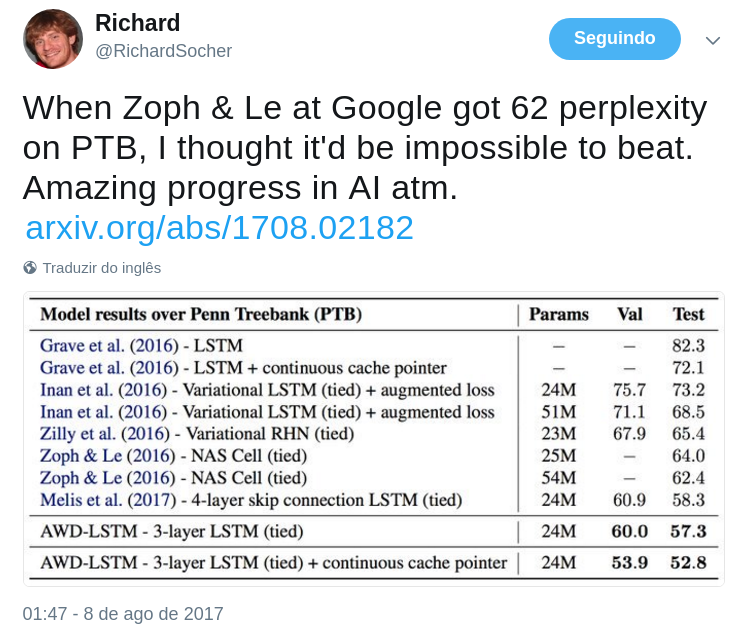
\includegraphics[scale=0.34]{images/SocherPTB.png}
\end{center}
\end{frame}

\begin{frame}
\begin{center}
\textbf{\LARGE{Obrigado!}}
\end{center}

\vspace{0.3cm}

\begin{center}

\includegraphics[scale=0.15]{images/gliclogo.pdf}
\end{center}
\url{https://glicusp.wordpress.com/}

\vspace{0.3cm}

\begin{center}

\includegraphics[scale=0.3]{images/logo0.pdf}
\end{center}
\url{https://www.ime.usp.br/~liamf/}

\end{frame}


\begin{frame}[allowframebreaks]{References}

  \bibliography{my_references}
  \bibliographystyle{abbrv}

\end{frame}

\end{document}